
\documentclass[12pt]{article}

\usepackage{lineno}


\usepackage[hmargin=1.5cm,vmargin=1.5cm]{geometry}

\usepackage[affil-it]{authblk}
\usepackage[percent]{overpic}
\usepackage{float}
\usepackage{color}
\usepackage{hyperref}
\usepackage[numbers,sort&compress]{natbib}

\title{Direct Tests of a Pixelated Microchannel Plate as the Active Element of a
Shower Maximum Detector}

\author[1]{A.~Apresyan}
\author[2]{S.~Los}
\author[1]{C.~Pena}
\author[1]{F.~Presutti}
\author[2]{A.~Ronzhin}
\author[1]{M.~Spiropulu}
\author[1]{S.~Xie}
\affil[1]{California Institute of Technology, Pasadena, CA, USA}
\affil[2]{Fermi National Accelerator Laboratory, Batavia, IL, USA}

\date{}

\begin{document}
\linenumbers

\maketitle
\abstract{One possibility to make a fast and radiation resistant shower maximum
detector is to use a secondary emitter as an active element. We report our studies
of microchannel plate photomultipliers (MCPs) as the active element of a
shower-maximum detector. We present test beam results obtained using Photonis
XP85011 to detect secondary particles of an electromagnetic shower. We focus on
the use of the multiple pixels on the Photonis MCP in order to find a transverse
two-dimensional shower distribution. A spatial resolution of 0.8 mm was obtained
with an 8 GeV electron beam. A method for measuring the arrival time resolution
for electromagnetic showers is presented, and we show that time resolution better than 40 ps can be achieved.}




\section{Introduction}

In order to collect large datasets needed for precise characterization of the
Higgs boson, and in order to increase new physics discovery potential, future
high-energy hadron colliders, as well as the High Luminosity LHC (HL-LHC)
upgrades are expected to deliver peak luminosities in excess of $5\times
10^{34}$~cm$^{-2}$s$^{-1}$. With the increased instantaneous luminosity the
simultaneous interactions per bunch crossing (pileup) increase the likelihood of
confusion in the reconstruction of particles from the hard scatter interaction
with those produced in different pileup interactions. The ability to
discriminate jets, photons, and electrons produced in the events of interests
from pileup becomes significantly degraded. One way to mitigate the pileup
confusion effects, complementary to precision tracking methods, is to perform a
time of arrival measurement associated with a particular layer of the
calorimeter, allowing for a time assignment for charged particles and photons.
In this paper we continue our investigation of the development of calorimeter
and shower-max detectors capable to measure the arrival time of
electromagnetically interacting
particles~\cite{Anderson:2015gha,MCPFastCaloNIMA,Ronzhin:2015pba,Ronzhin2015288}. 

Past studies have indicated that using micro-channel plates (MCP) as the active
element of a shower-maximum detector or a calorimeter is a promising option for
achieving time measurement precision at the level of a few tens of
picoseconds~\cite{MCPFastCaloNIMA,Ronzhin:2015pba,Ronzhin2015288,Brianza2015216}. Moreover,
such devices are intrinsically radiation hard and thus would tolerate the harsh
radiation environment at future hadron colliders. A further advantage of MCP's
is their capability for highly segmented readout, allowing for the possibility of a
highly granular calorimeter with sub-millimeter spatial resolution. Such
high-granularity calorimeters have been studied in the context of detector
concepts for the ILC~\cite{Grondin:2010fe} and the HL-LHC upgrade of the CMS 
experiment~\cite{Butler:2020886}, indicating that such calorimeters have promising 
potential for substantial improvement in physics reach at the TeV scale.

In this and the three previous papers we used three different MCP-PMTs:
\begin{itemize}
\item Photek 240: this is our highest performant device, which provides the best
      time resolution, and good uniformity across the detector. Main parameters
      of the Photek 240 were reported in Ref.~\cite{MCPFastCaloNIMA}. The pore
      size is 10~$\mu$m and the distance from the photocathode to the first
      amplification stage is 5.3~mm. The Photek 240 has a 41~mm$^2$ circular
      sensitive area, and it was operated 4.8~kV high voltage (HV). The gain at
      this voltage is about 10$^6$. The output signal time shift is limited to
      3.9~ps across the sensitive area of the Photek 240.
\item Photonis XP85011: the anode of this MCP is composed of 64 pads, arranged
      as an $8\times8$ matrix. The size of each pad is 6×6 mm2. The pore size of the
      Photonis MCP-PMT is 25 μm. Timing non-uniformity across the photocathode
      is 37 ps when using the passive sum of 16 pads~\cite{MCPFastCaloNIMA, Ronzhin2015288}. The
      HV applied to the tube Photonis XP85011 was 2.4~kV, with a corresponding
      gain of $10^6$. 
\item Photonis XP85012: like XP85011 is also composed of 64 pixels, arranged as
      an $8\times8$ matrix. The charactersitcs of this device are the same as
      those for Photonis XP85011, and additionally it can be operated in a mode
      when reverse voltage is applied to photocathode, which enables us to turn
      the photocathode OFF, in order to measure the direct signals from
      secondary showers~\cite{Ronzhin:2015pba}.  
\end{itemize}


In this paper, we report our studies of a high-granularity shower-maximum
detector that uses the Photonis XP85011 MCP as the active element to detect
direct secondary emission particles. The MCP is used to sample the
electromagnetic shower induced by a beam of electrons impacting a tungsten
absorber layer that has a thickness of about 4 radiation lengths ($X_{0}$). The
MCP-PMT is read out with a pixelated anode, with square pixels of size $6$~mm.
The energy of the electromagnetic showers is reconstructed using the total
collected charge and the positions are reconstructed using a simple
energy-weighting algorithm, described in Section~\ref{sec:position}.
Through the use of a high-precision motorized stage, a position scan is
performed during beam-tests and the position resolution of the shower-maximum
detector is obtained. Finally, we investigate the precision of measuring the
arrival time of electromagnetic showers with such a pixellated shower-maximum
detector.

The paper is organized as follows. In Section~\ref{sec:setup} we describe the
experimental setup used to perform the measurements, in
Section~\ref{sec:reconstruction} we present the event selection and pulse
reconstruction, in Section~\ref{sec:position} and~\ref{sec:timing} the results
on measured position and timing resolutions are presented. 

\section{Experimental Setup} \label{sec:setup} The experiment was performed at
the MTEST location of the Fermilab Test Beam Facility using an $8$~GeV beam
primarily comprised of electrons. A differential Cherenkov counter, located
further upstream of the MTEST location, was used to enhance the purity of
electrons and to suppress pions, by requiring a signal consistent with a passage
of electrons through the counter. All other detectors were placed inside a dark
box lined with copper foil for electromagnetic shielding. A photograph of the
experimental setup within the dark box is shown in Figure~\ref{fig:setup}. A
scintillator of size $1.7$~mm$\times$~$2.0$~mm optically coupled to two
photomultiplier tubes, one on each side, was used to trigger the data
acquisition and to constrain the trajectory of the electrons from the beam.
Downstream of the trigger, a tungsten absorber with a thickness of about $1$~cm,
equivalent to about 4 radiation lengths, was placed. The Photonis XP85011
MCP-PMT with pixelated readout was set on a high precision motorized stage and
placed behind the tungsten absorber. The precision of the motorized stage is
about $0.1$~mm. To avoid unintended early showers due to interactions with the
material of the casing and MCP device, the Photek 240 MCP-PMT was placed behind
the Photonis XP85011 MCP-PMT. 

\begin{figure}[htbp] 
\centering
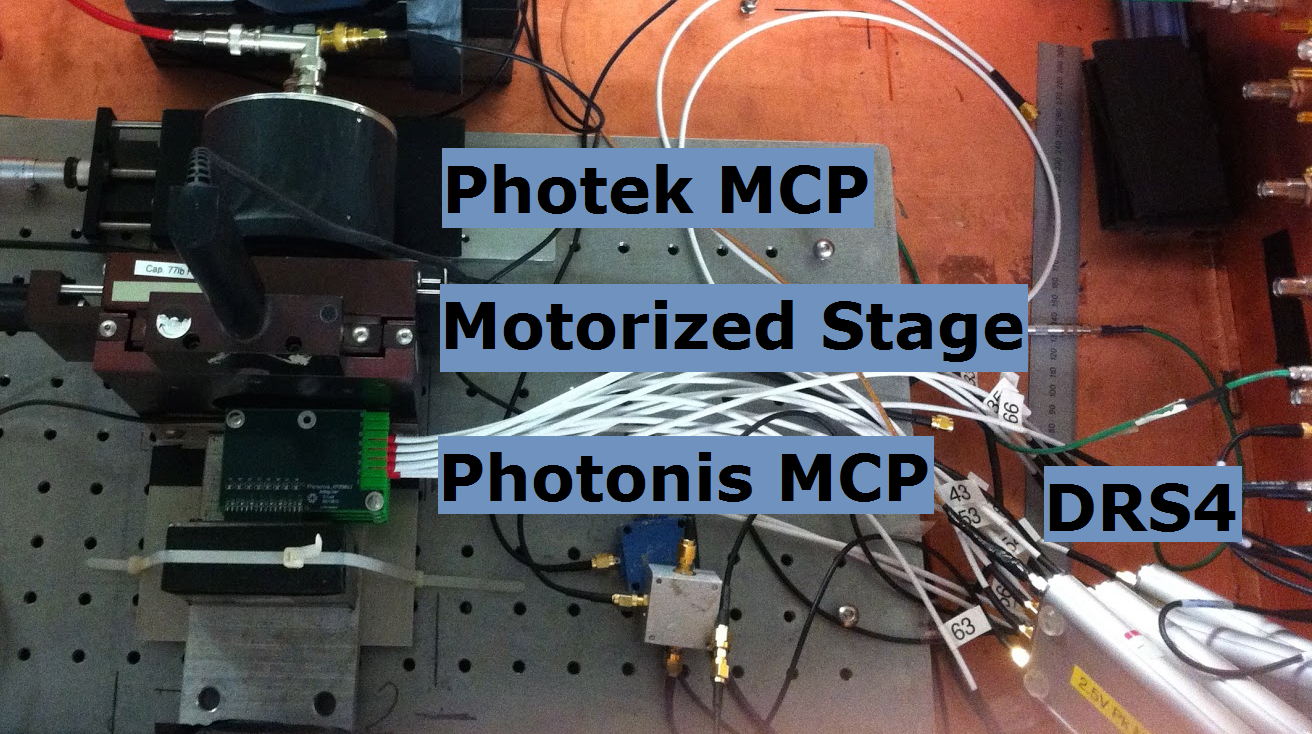
\includegraphics[width=0.8\textwidth]{Images/setup/setup.png} 
\caption{The experimental setup inside of the dark box is shown. The beam direction is from
the bottom of the photograph to the top. The detector elements shown in the
order from upstream to downstream of the beam are: the tungsten absorber, the
Photonis XP85011 MCP-PMT located on the motorized stage, and the Photek 240
MCP-PMT used as a time reference detector. The DRS4 waveform digitizers are also
shown on the lower right side.} 
\label{fig:setup} 
\end{figure} 

An external view
of the Photonis XP85011 MCP-PMT is shown on the left of Figure~\ref{fig:photonis},
and a schematic diagram is shown on the right. There are a total of 64 pixels
arranged in an $8\times8$ square that can be read out individually. For our
experiment, the nine pixels shown within the red square are used. During the
course of the experiment we found that the pixel labelled 44 in
Figure~\ref{fig:photonis} did not function properly and was therefore not used
in the analysis of the data. 

\begin{figure}[htbp] 
\centering
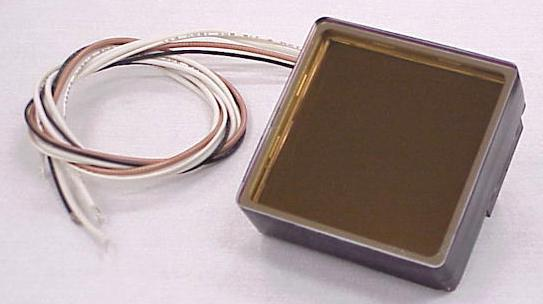
\includegraphics[width=0.49\textwidth]{Images/photonis/photonis.jpg}
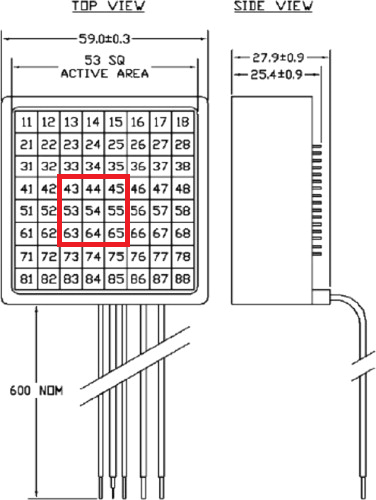
\includegraphics[width=0.49\textwidth]{Images/photonis/photonis2.png}
\caption{The external view of the Photonis XP85011 MCP-PMT is shown on the left, and
the schematic diagram is shown on the right. The red square indicates the pixels
used for the experiment and data analysis.} 
\label{fig:photonis} 
\end{figure}

Four DRS4 high speed waveform digitizers were used to acquire the signals from
the Photek 240 MCP-PMT, the cherenkov counter, and the eight operational
channels from the Photonis XP85011 MCP-PMT. In order to allow a synchronized
readout of four separate DRS4 units we split the signals from the Photek 240
MCP-PMT into four, and connected them to each of the four DRS4 units, thus achieving
a ``calibration'' between the four different units.  

% should draw a diagram of how the channels were distributed among the 4 DRS %units


\section{Event Selection and Pulse Reconstruction}
\label{sec:reconstruction}
Reconstruction of the signal pulses and timestamps is performed using the
identical methods described in our past
studies~\cite{Anderson:2015gha,MCPFastCaloNIMA,Ronzhin:2015pba}.
In Figure~\ref{fig:expulse}, we show example pulses from one pixel channel of
the Photonis XP85011 MCP-PMT and the Photek 240 MCP-PMT digitized by the DRS4.


We measure time resolution as the standard deviation of the Gaussian fit to the
time-of-flight distribution $t_0-t_1$, where $t_0$ is the time recorded at the
``start'' detector, and $t_1$ is that of the ``stop'' detector. To assign a time
stamp for each signal pulse, we first determine the time position of the pulse
peak. A Gaussian function is fitted to the pulse maximum using three points
before the maximum of the pulse peak and four points after the maximum. The mean
value of the Gaussian was used as the time stamp for each pulse. A Photek 240
MCP-PMT, whose time resolution was previously measured to be less than
$10$~ps~\cite{Ronzhin:2015pba} was used as a ``start'' signal, while pulses from
individual pixels on the Photonis XP85011 MCP-PMT were used as ``stop'' signals.
More details on the pulse reconstruction algorithms that we use are presented in
Ref.~\cite{MCPFastCaloNIMA}. The integrated charge for each pulse is used as a
proxy for the measured energy deposit in each channel, and is computed using
four time samples before and after the peak of the pulse. Each time sample is
approximately $0.2$~ns in time. Events containing pulses above $500$~mV in
amplitude are rejected as they saturate the DRS4. Only pulses with amplitude
larger than $20$~mV are used for time measurements, to reduce the impact of the
electronics noise in the DRS4. Other event selection and pulse cleaning
procedures are used to eliminate abnormal pulses in the readout, as described
in~\cite{MCPFastCaloNIMA}. 

\begin{figure}[htbp]
	\centering
	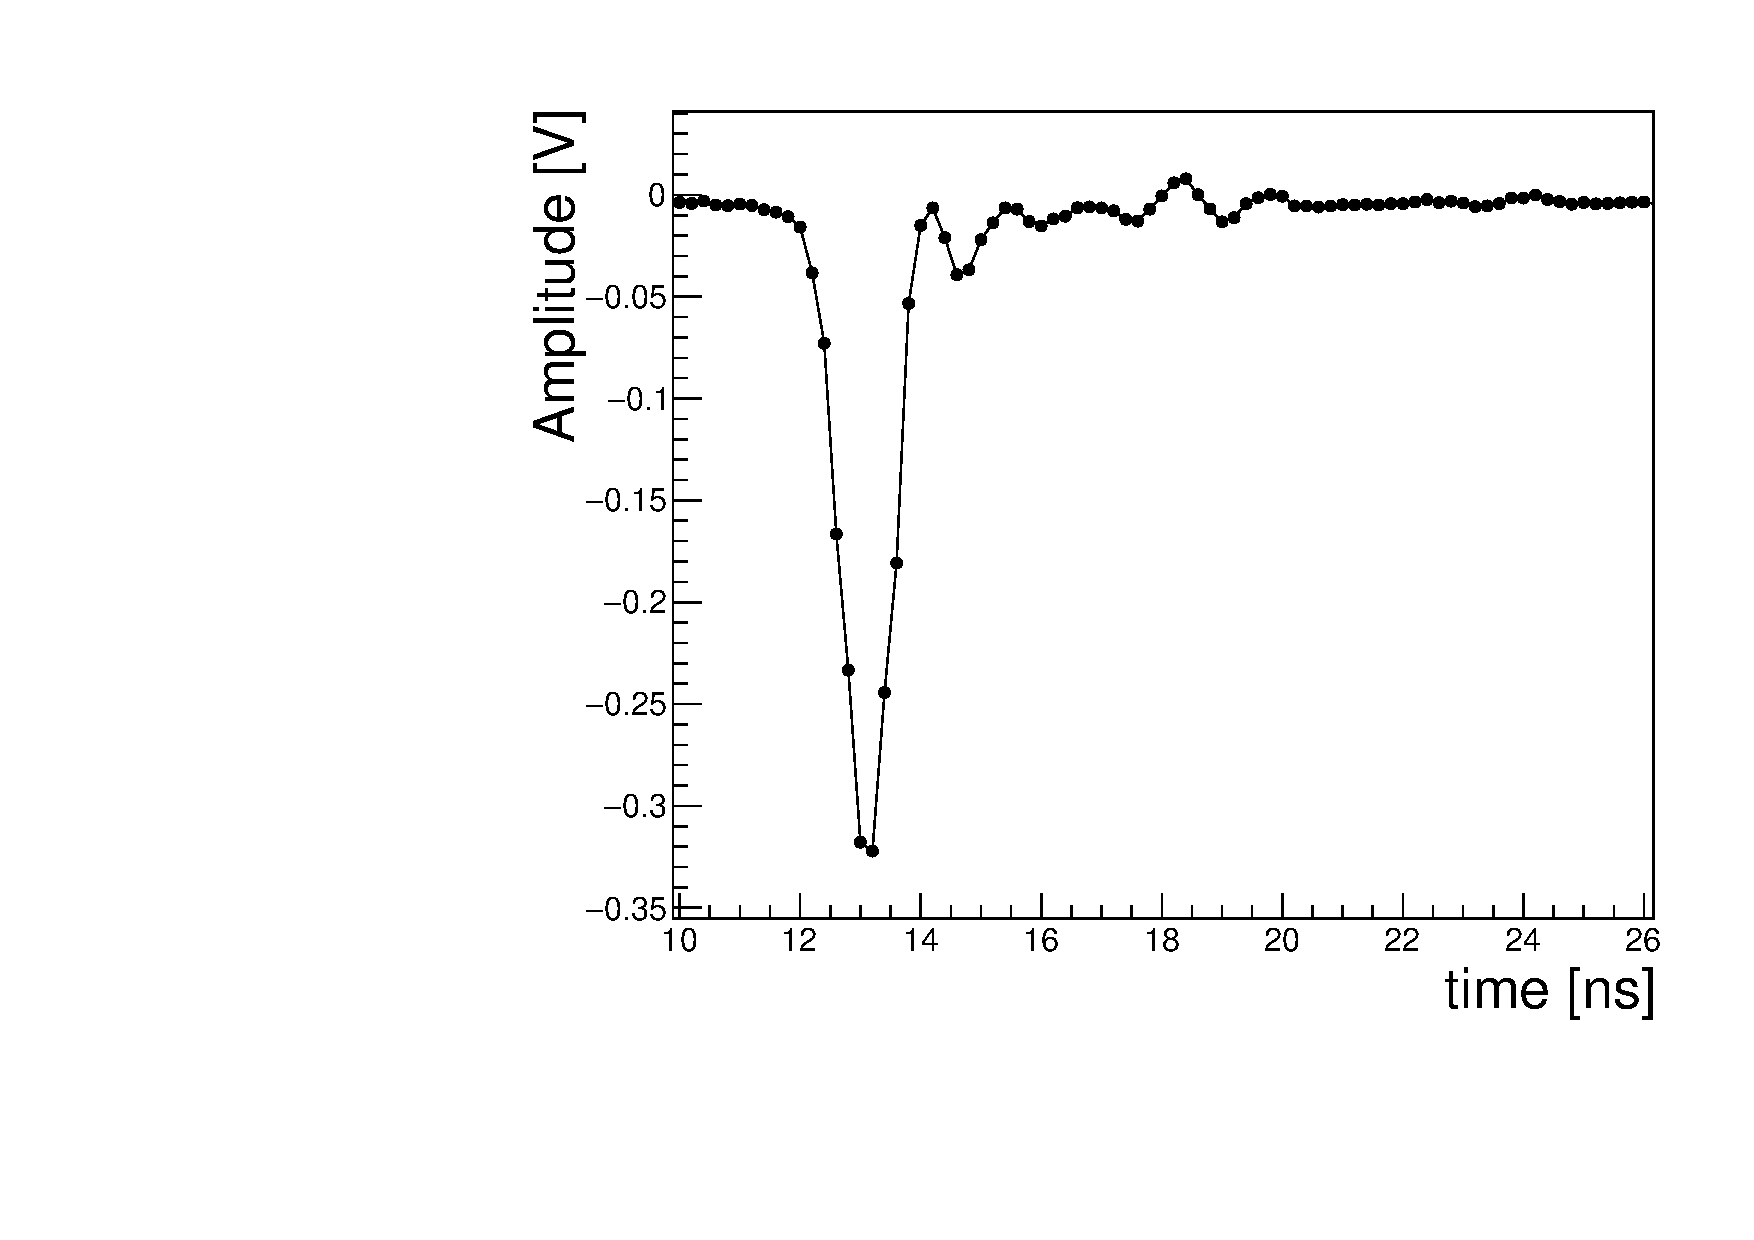
\includegraphics[width=0.49\textwidth]{Images/expulse/pulsepix_30_2_12.pdf}
	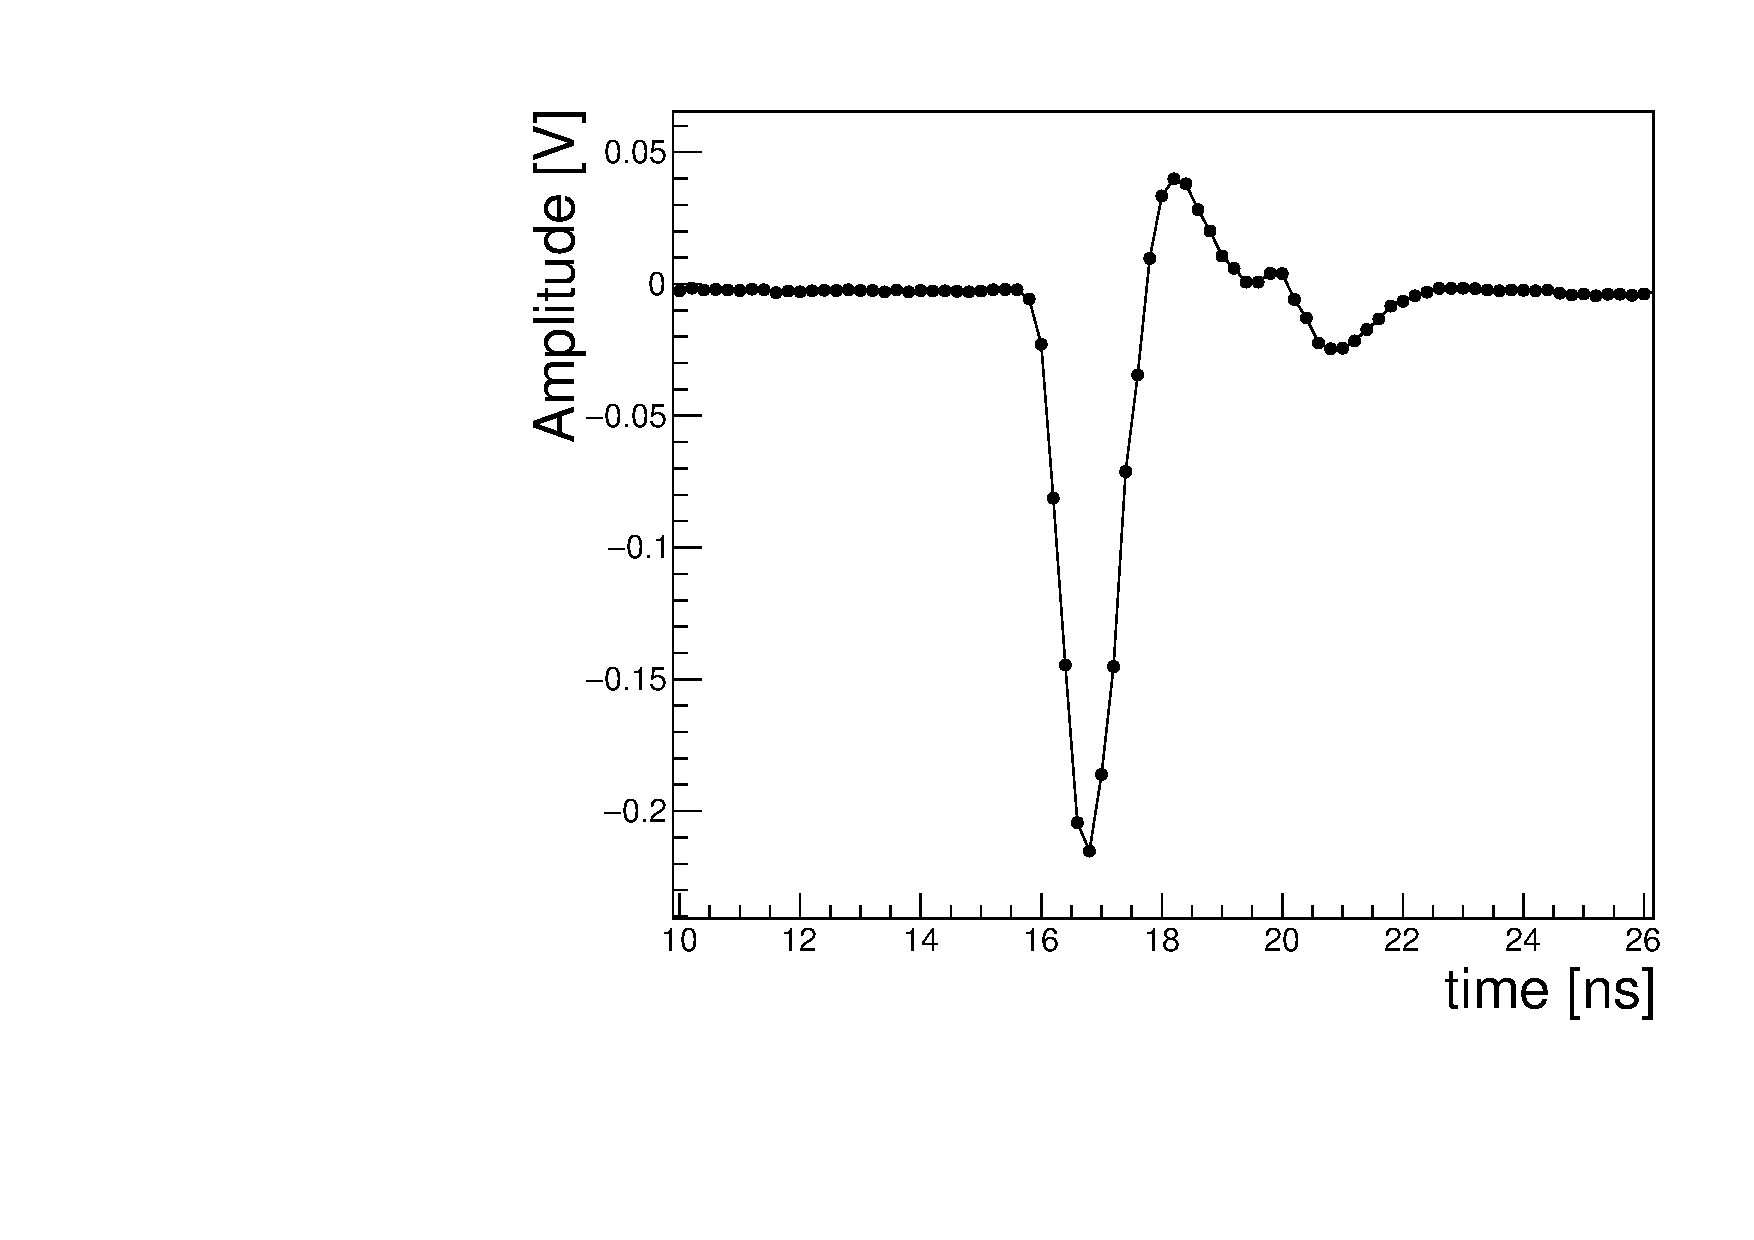
\includegraphics[width=0.49\textwidth]{Images/expulse/pulseref_30_2_10.pdf}
	\caption{\small Example of a digitized signal from a single Photonis pixel
(left) and Photek (right) MCP-PMT following a high-energy electron shower, via DRS4.}
	\label{fig:expulse}
\end{figure}


\section{ Electromagnetic Shower Position Reconstruction and Resolution}
\label{sec:position} The transverse shape of electromagnetic showers is very
well known and has a characteristic width given by the Moliere radius. For
tungsten, the Moliere radius is about $9$~mm and therefore we expect the shower
to be contained within two of the pixels in the Photonis XP85011 MCP-PMT. In
Figure~\ref{fig:exavint}, we show the mean charge measured in each of the pixels
for one example run where the Photonis MCP-PMT was held in a fixed location
approximately centered on the beam. The electron beam has a width of about
$1$~cm. 

\begin{figure}[htbp] 
\centering
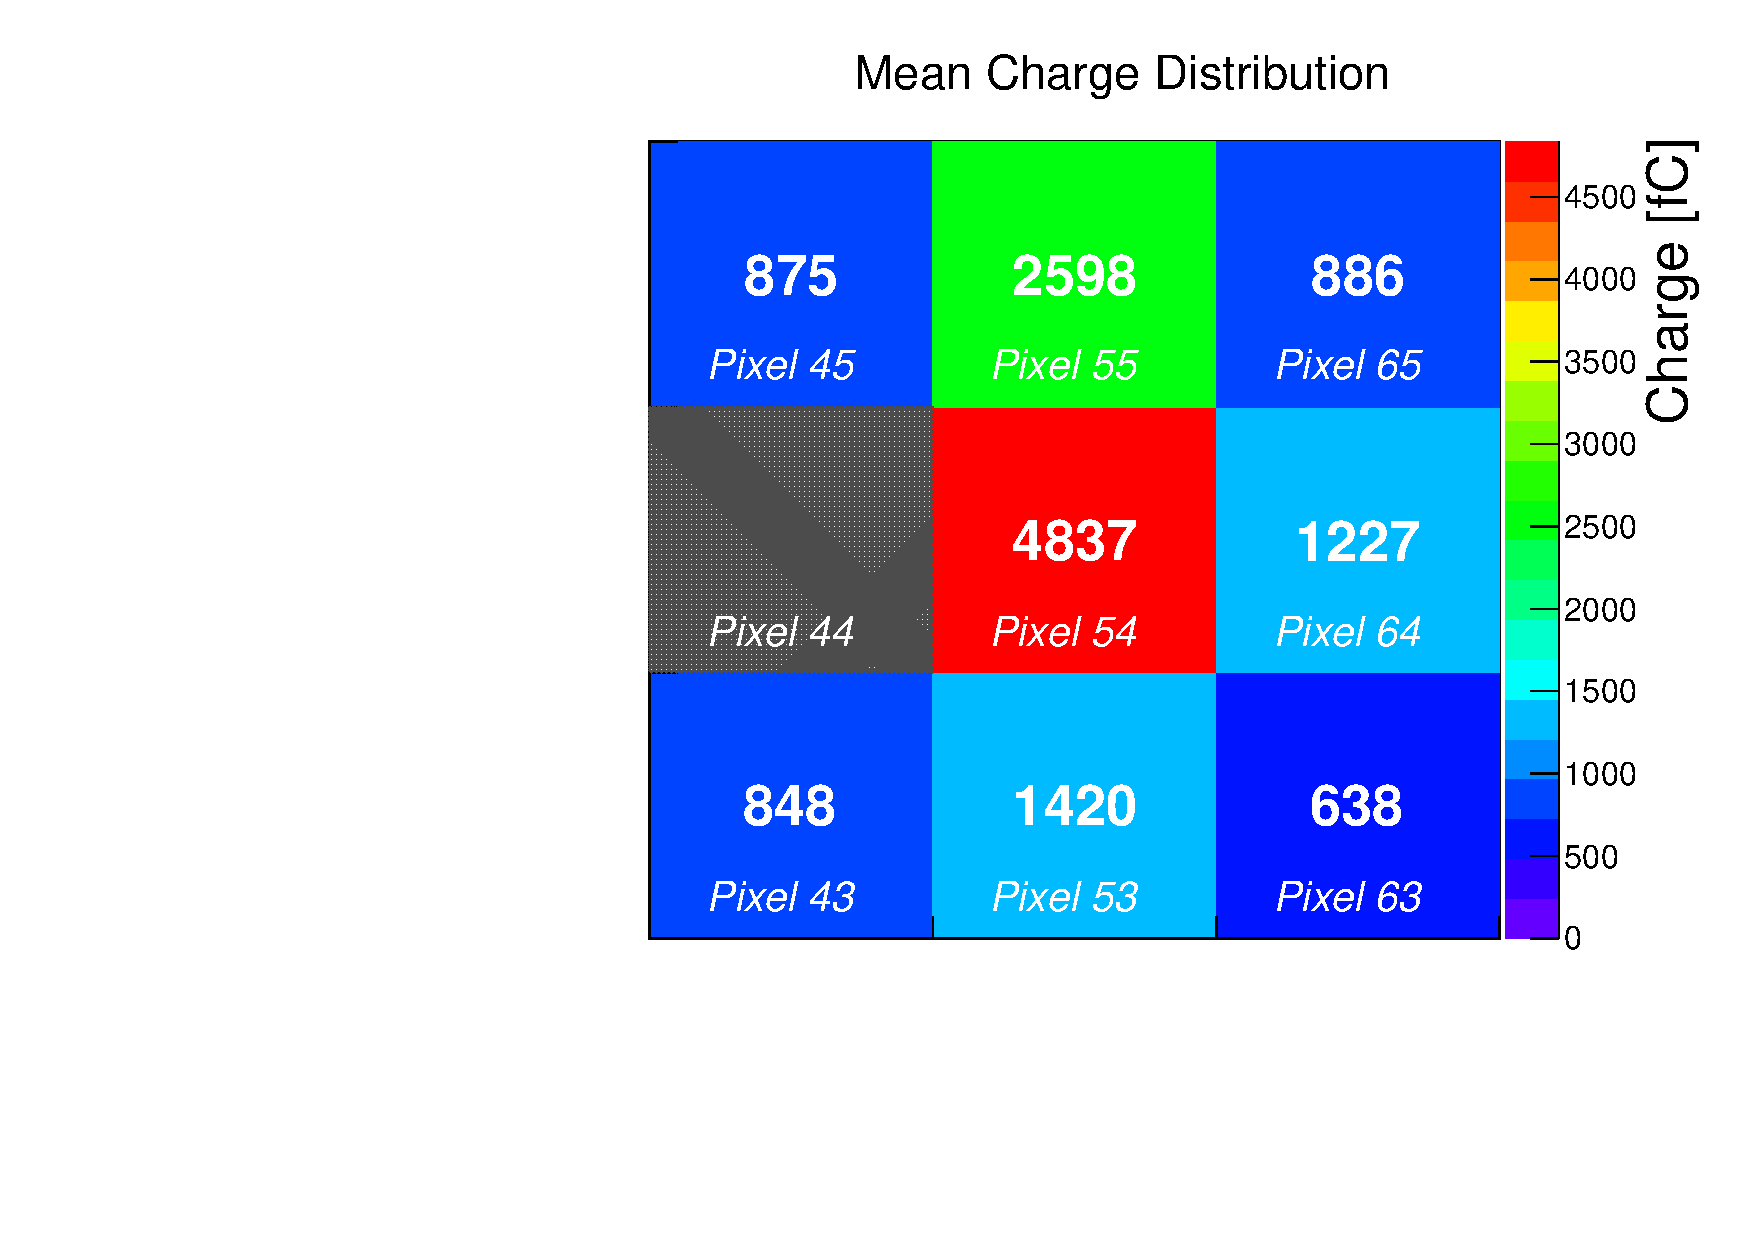
\includegraphics[width=8cm]{Images/exavint/exintrun30.pdf} 
\caption{\small The mean charge measured for each pixel for one example run is shown. During this run, the Photonis MCP-PMT was held in the same location. Based on the distribution
of the mean charge among the pixels, we can infer that the beam center is
located in the upper half of the center pixel. Pixel 44 is not shown as it was
found to be not operational. } 
\label{fig:exavint} 
\end{figure} 

Each electron impacting the shower-maximum detector will induce an
electromagnetic shower, and we define such an occurrence as an event. For each
event, we reconstruct the center position, $\vec{p}$ of the electromagnetic
shower based on the the pixel positions weighted by the corresponding integrated
charge as follows: 
\begin{equation} 
 \vec{\mathbf{{p}}} =
\frac{\sum_{i\in\mathrm{pixels}} Q_{i} \vec{p}_i} {\sum_{i\in\mathrm{pixels}}
Q_{i}} 
\end{equation} 

where $i$ labels the individual pixels, $Q_{i}$ is the charge collected in pixel
$i$, and $\vec{p}_{i}$ is the vector describing the $x$ and $y$ coordinates of
the center of pixel $i$. The origin of the coordinate system is chosen to be at
the lower left corner of the $3\times3$ array of pixels.

Multiple runs were taken scanning different beam positions relative to the
Photonis MCP-PMT by moving the motorized stage. In
Figure~\ref{fig:EMShowerPositions} we show the distributions of the
reconstructed shower positions for three example runs in which the beam was
located near the top, center, and bottom of the center pixel. The distributions
of the reconstructed $y$ coordinate for the three corresponding runs are shown
together in Figure~\ref{fig:EMShowerYPositionComparison}. The measured beam-spot
is observed to move consistent with the known movement of the motorized stage.

\begin{figure*}[htbp] \centering
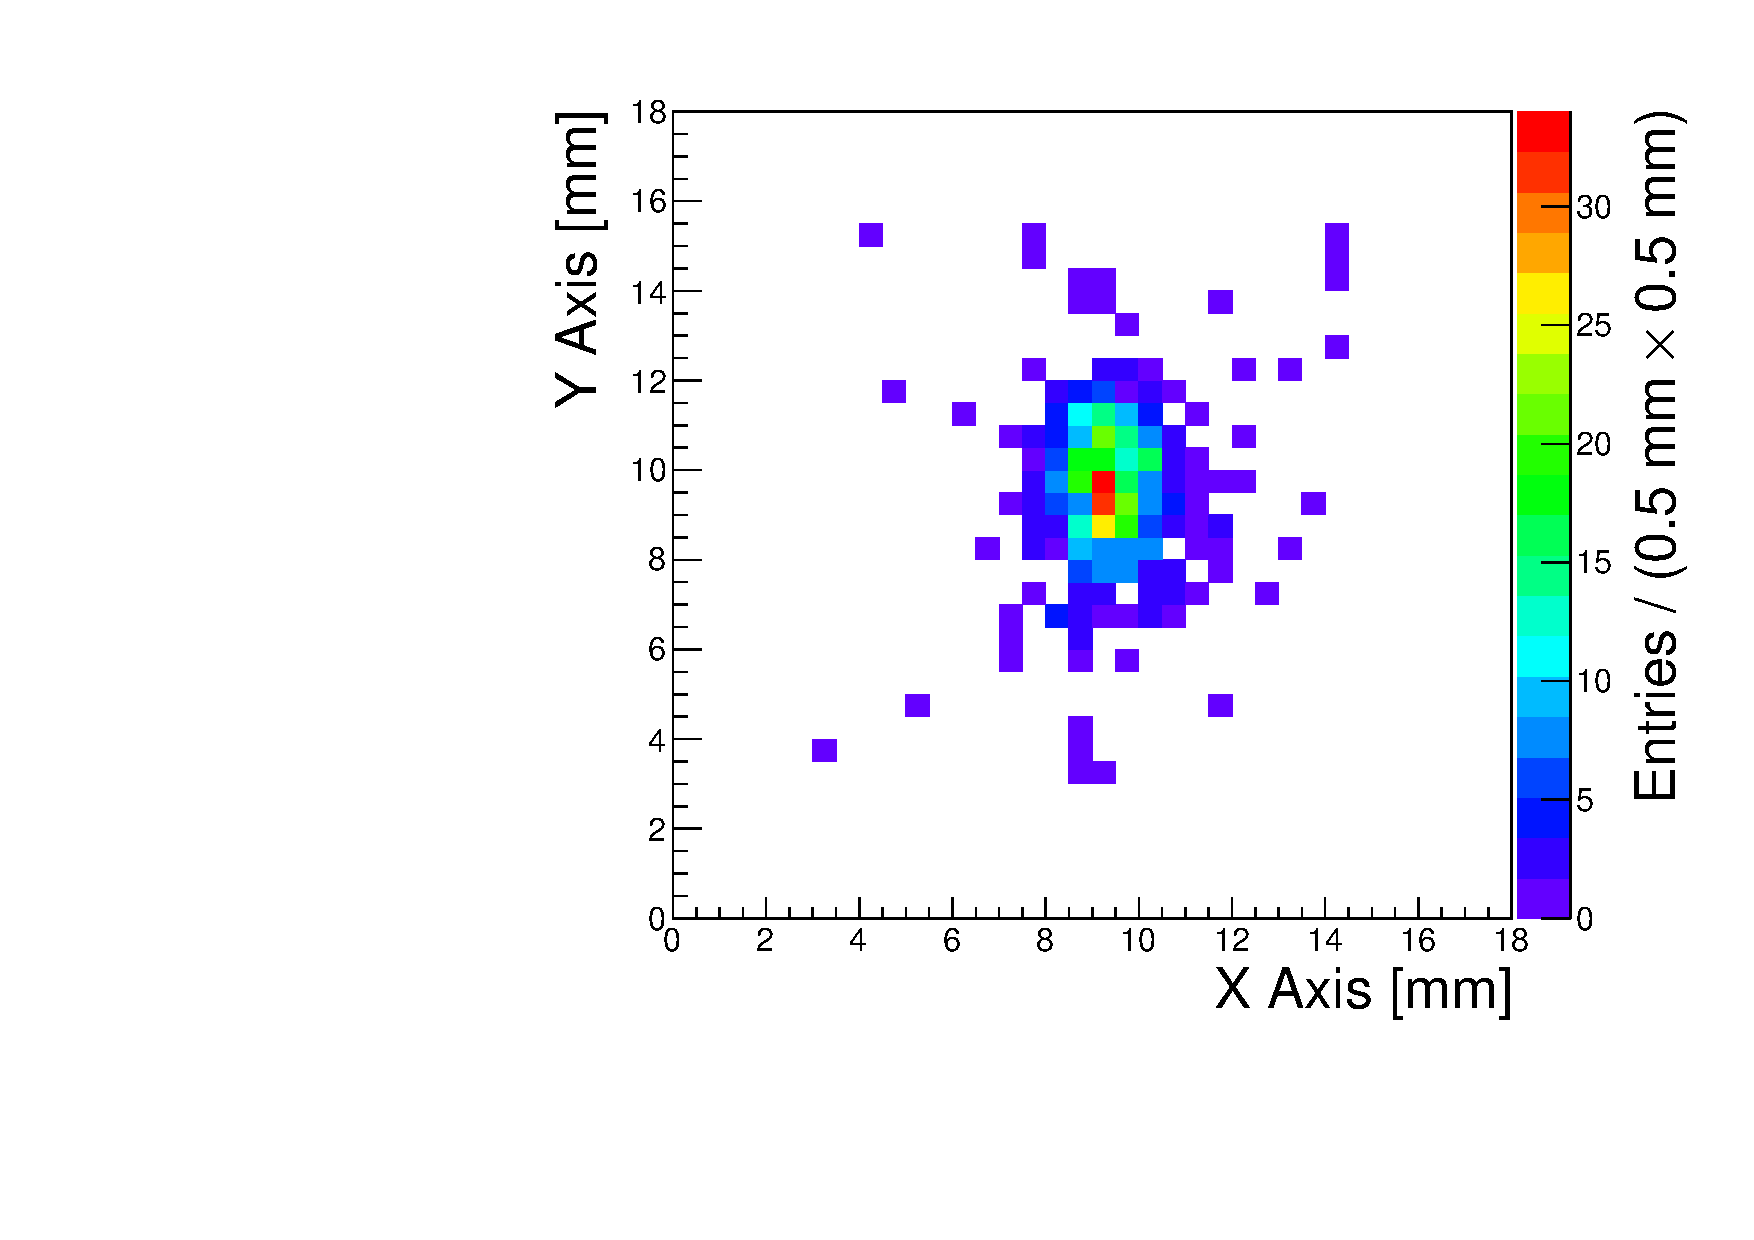
\includegraphics[width=0.49\textwidth]{Images/centers/run30dist.pdf}
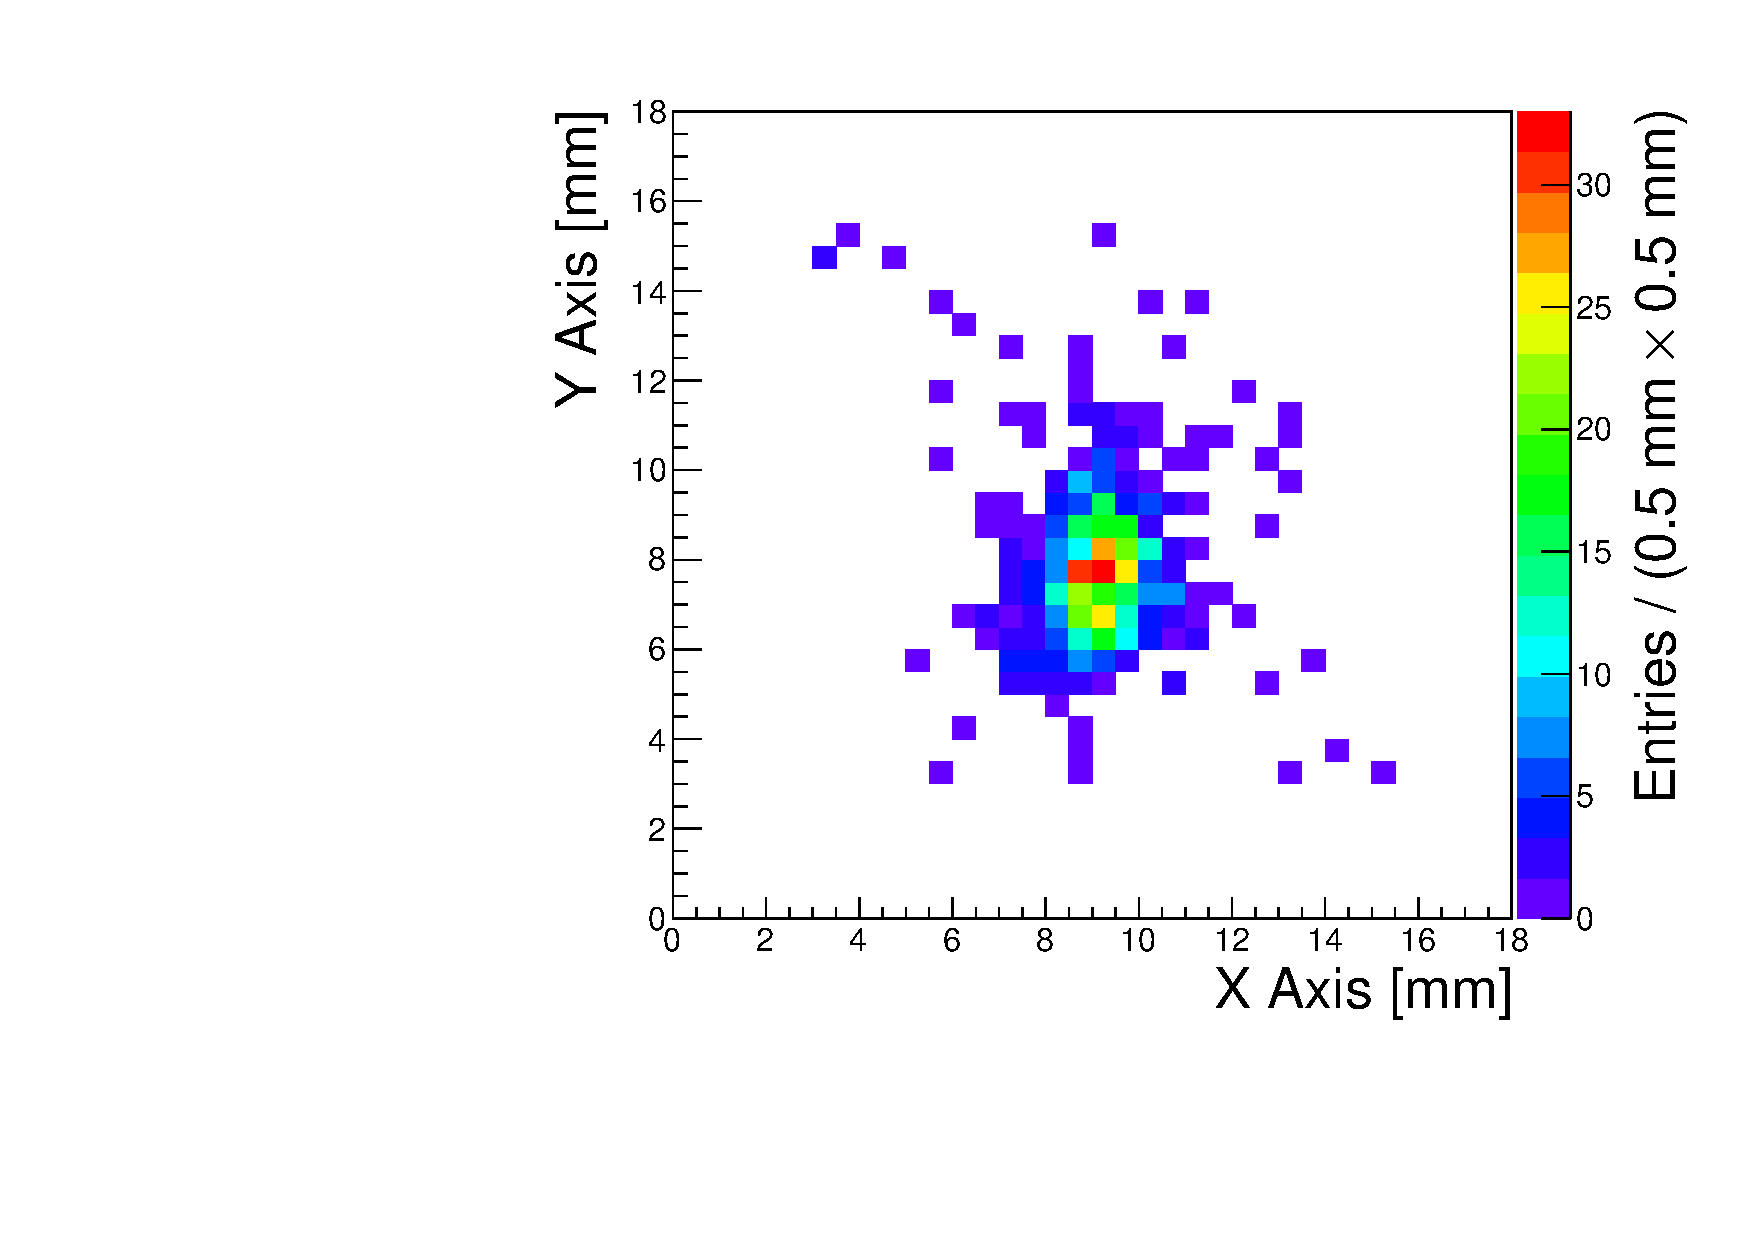
\includegraphics[width=0.49\textwidth]{Images/centers/run32dist.pdf}
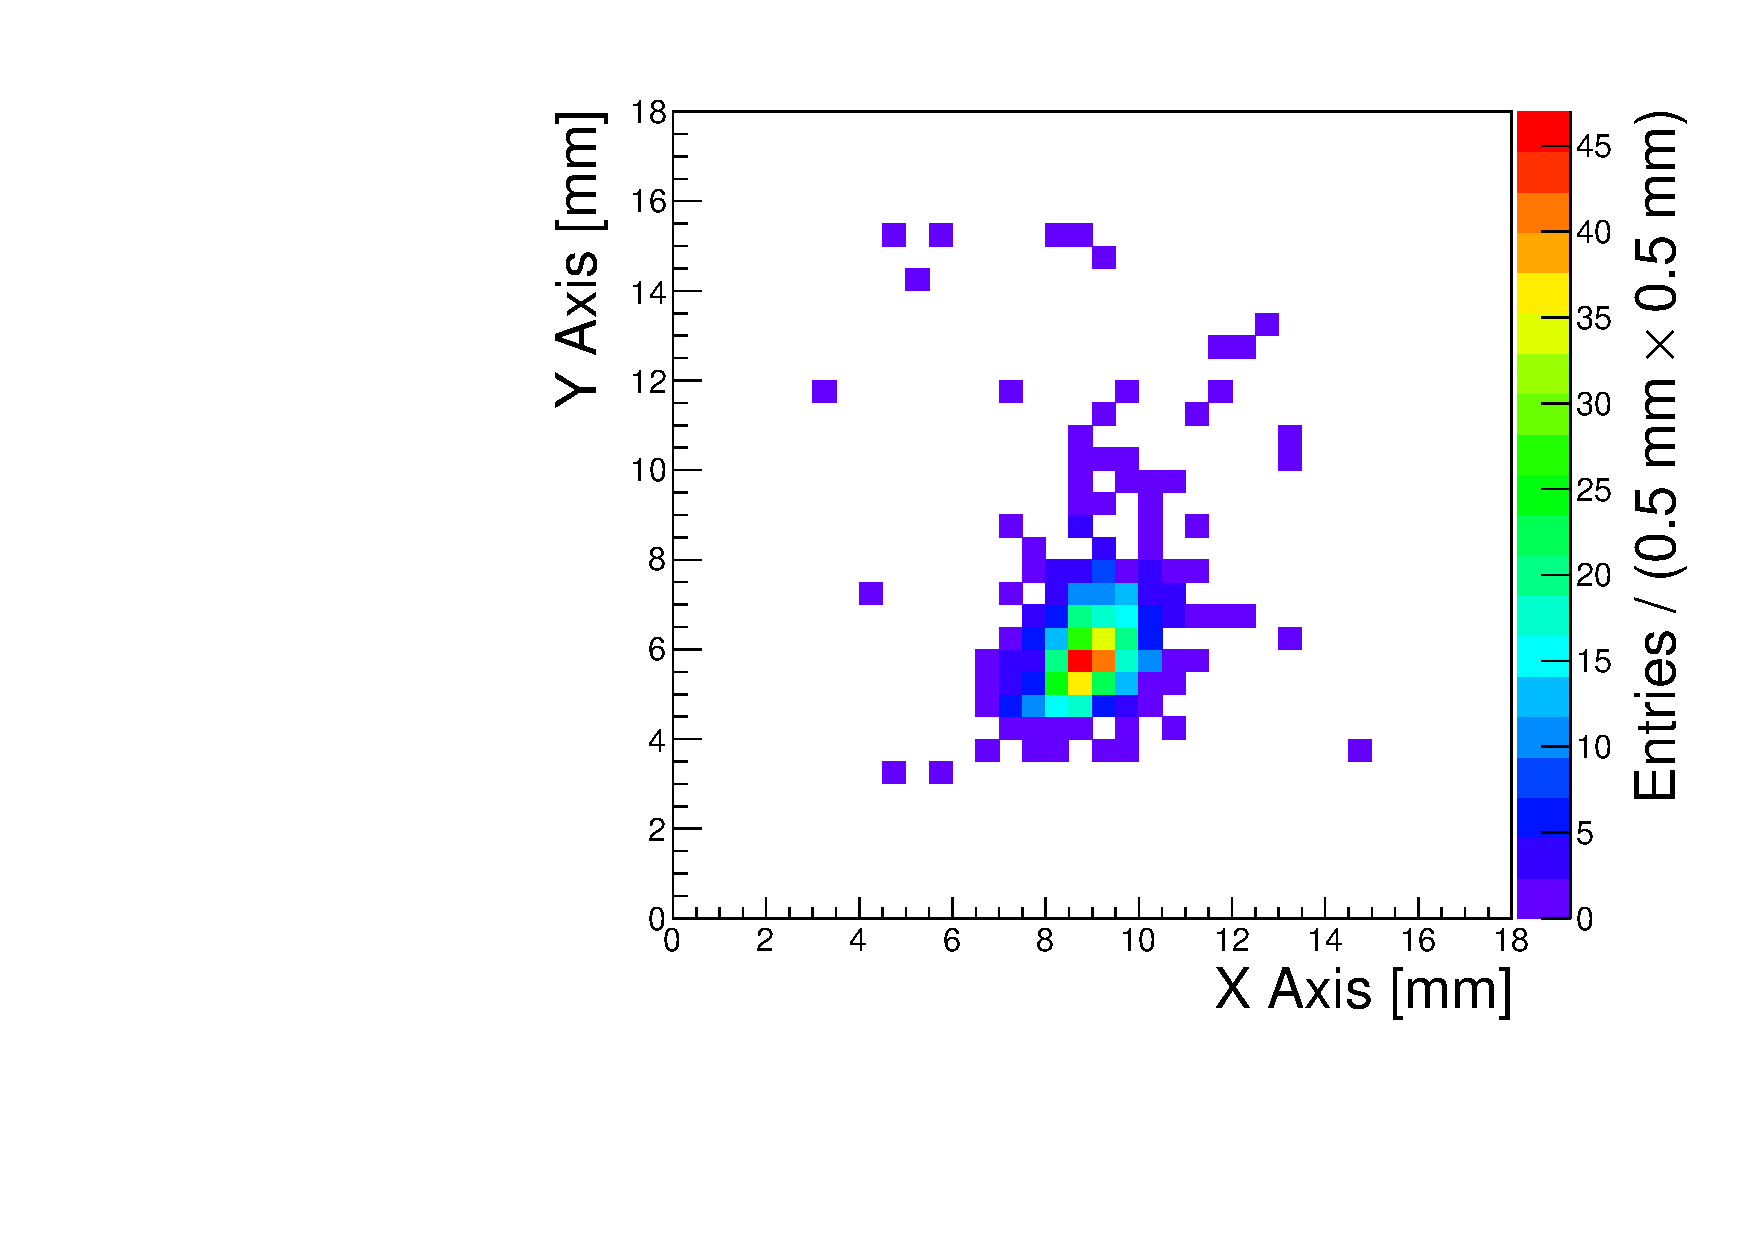
\includegraphics[width=0.49\textwidth]{Images/centers/run34dist.pdf}
\caption{The distribution of reconstructed shower positions is shown for three
runs with the beam centered near the top, center, and bottom of the central
pixel. } \label{fig:EMShowerPositions} \end{figure*} \begin{figure*}[htbp]

\centering
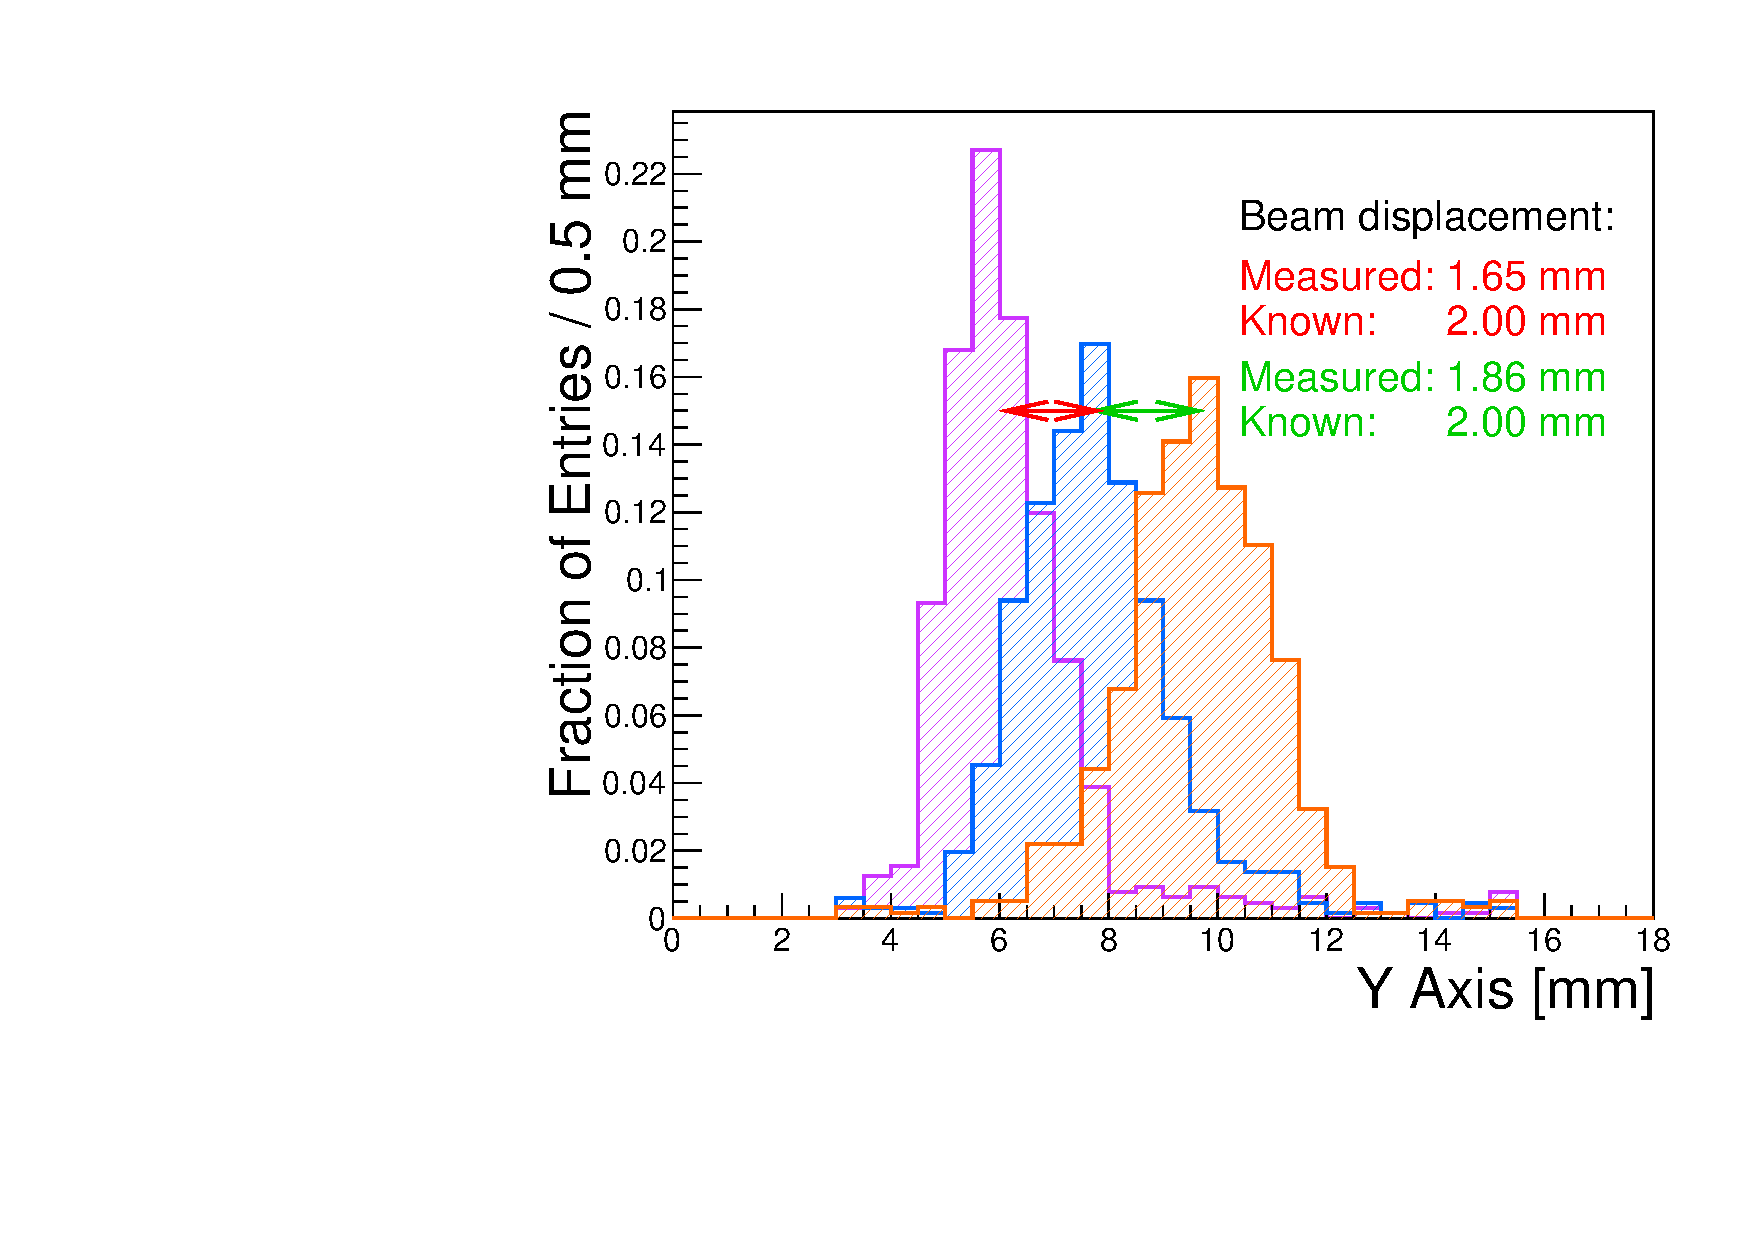
\includegraphics[width=0.75\textwidth]{Images/centers/superimposed.pdf}
\caption{The distributions of reconstructed shower position in the $y$ axis is
shown for the three runs corresponding to the distributions shown in
Figure~\ref{fig:EMShowerPositions}. The measured beam displacements are compared
to the known displacements as recorded by the motorized stage. }
\label{fig:EMShowerYPositionComparison} 
\end{figure*} 

For each run, we determine the center of the beam-spot by fitting the measured
$x$ and $y$ coordinates with a gaussian function. The data from all runs are
combined by considering the measured $x$ and $y$ coordinates relative to the
center of the beam-spot (see Fig~\ref{fig:ResolutionMeasurement}). We model the
distribution of measured coordinates as a convolution of a flat distribution
with width equal to the measured dimensions of the scintillator trigger and a
gaussian resolution function. A maximum likelihood fit is performed on the data
using this model, and the position resolution of the detector is measured as the
width of the gaussian resolution function. We measure the position resolution as
$0.55\pm0.2$~mm in $x$-coordinate, and $0.91\pm 0.01$~mm in $y$-coordinates.

\begin{figure*}[htbp] \centering
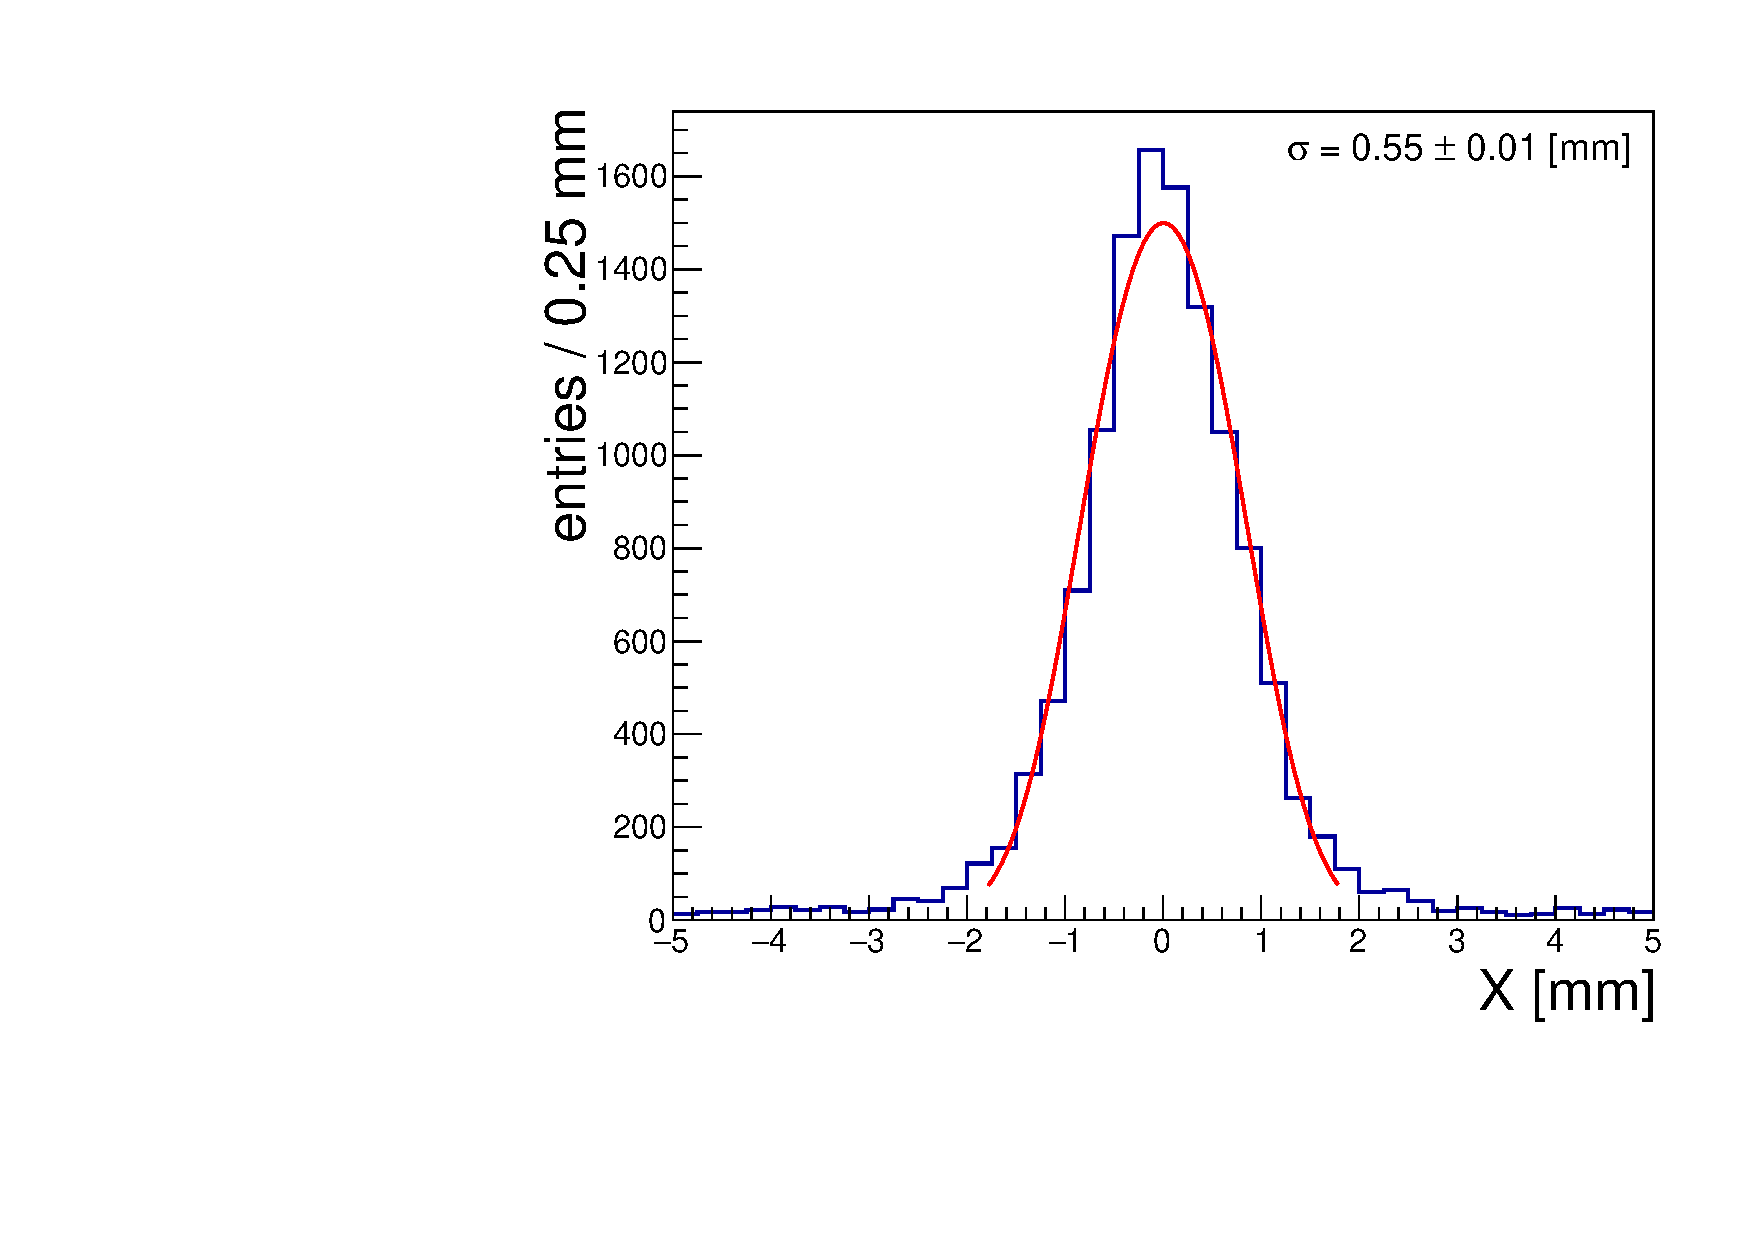
\includegraphics[width=0.49\textwidth]{Images/XYResolution/X_Resolution_fixedTrigger.pdf}
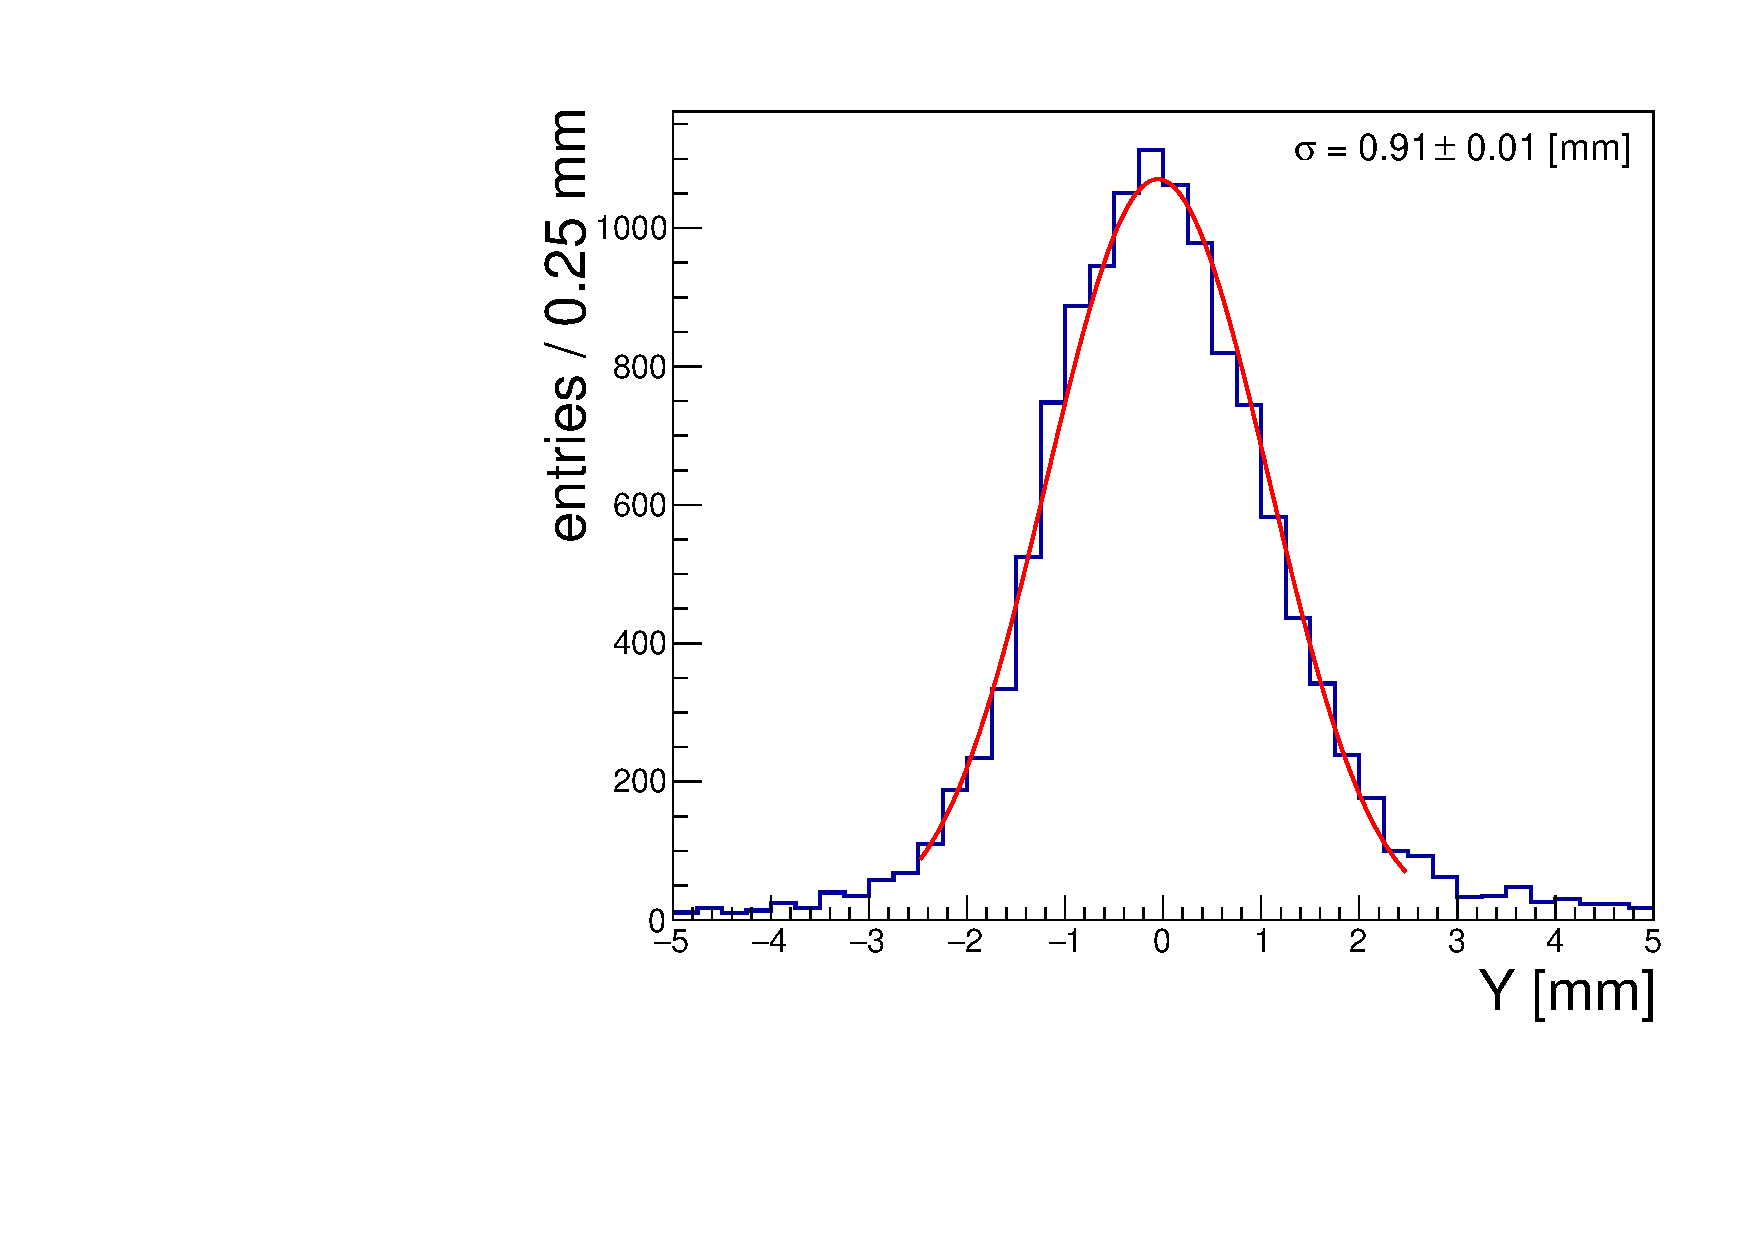
\includegraphics[width=0.49\textwidth]{Images/XYResolution/Y_Resolution_fixedTrigger.pdf}
\caption{The distributions of the measured $x$ (left) and $y$ (right)
coordinates are shown along with the fit to the resolution model. The position
resolution of the EM shower as measured by the MCP-PMT detector is determined from
the fit to the resolution model. } \label{fig:ResolutionMeasurement}
\end{figure*}

\section{ Electromagnetic Shower Time Resolution } 
\label{sec:timing} 

The timestamps for each event for individual pixels of the Photonis MCP-PMT are
reconstructed as described in Section~\ref{sec:reconstruction}. We reconstruct
the timestamp of the entire electromagnetic shower using the same energy
weighting procedure that was used above for the shower position reconstruction:

\begin{equation} t =\frac{\sum_{i\in\mathrm{pixels}} Q_{i} t_{i}}
{\sum_{i\in\mathrm{pixels} Q_{i}}}, 
\label{eqn:EnergyWeightedTimestamp}
\end{equation} 

where $i$ labels the individual pixels, $Q_{i}$ is the charge
collected in pixel $i$, and $t_{i}$ is the reconstructed time-stamp for pixel
$i$. Alternatively, we also study the time resolution using the single pixel
with the highest energy deposit measurement. In Figure~\ref{fig:exdt} we show
the time distributions for these two methods of shower time reconstruction.

\begin{figure*}[htbp] 
\centering
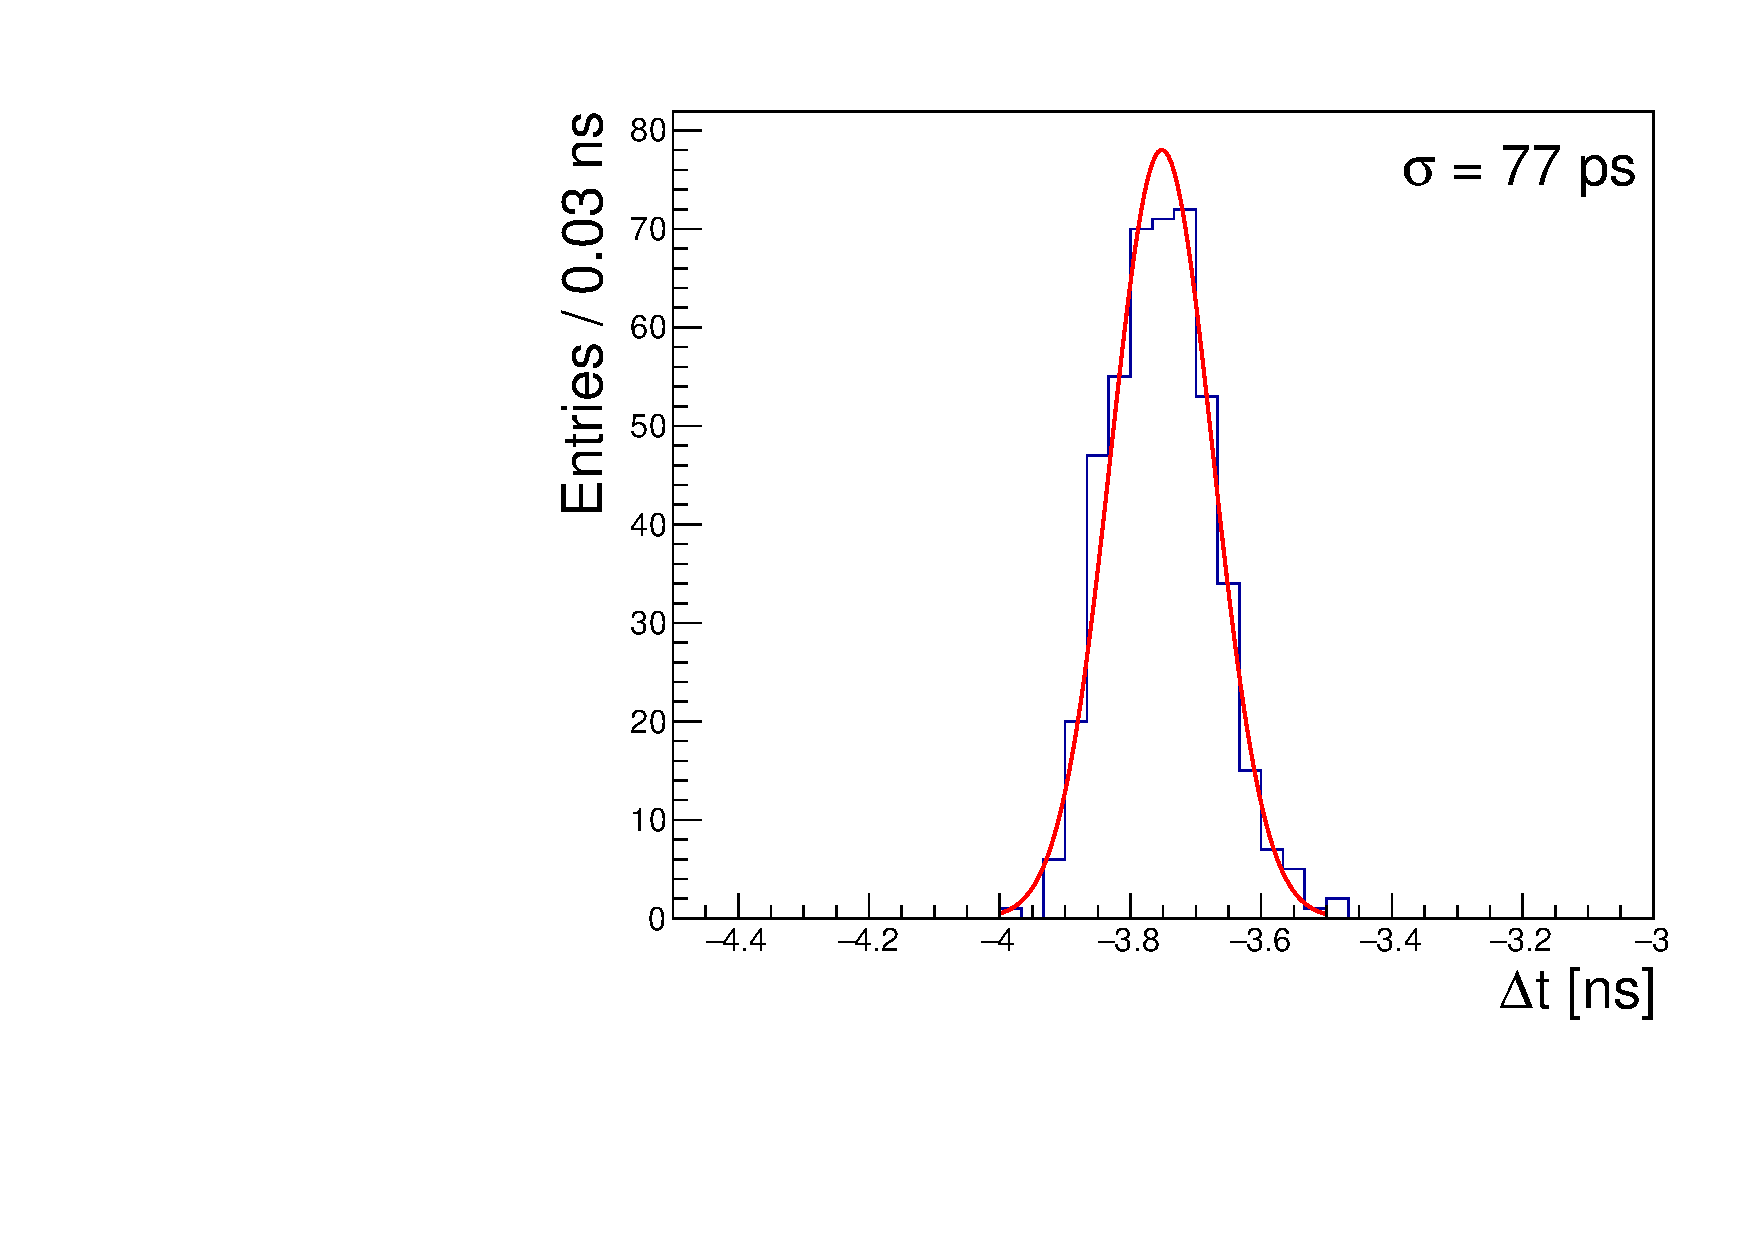
\includegraphics[width=8cm]{Images/exdt/exdtHI.pdf}
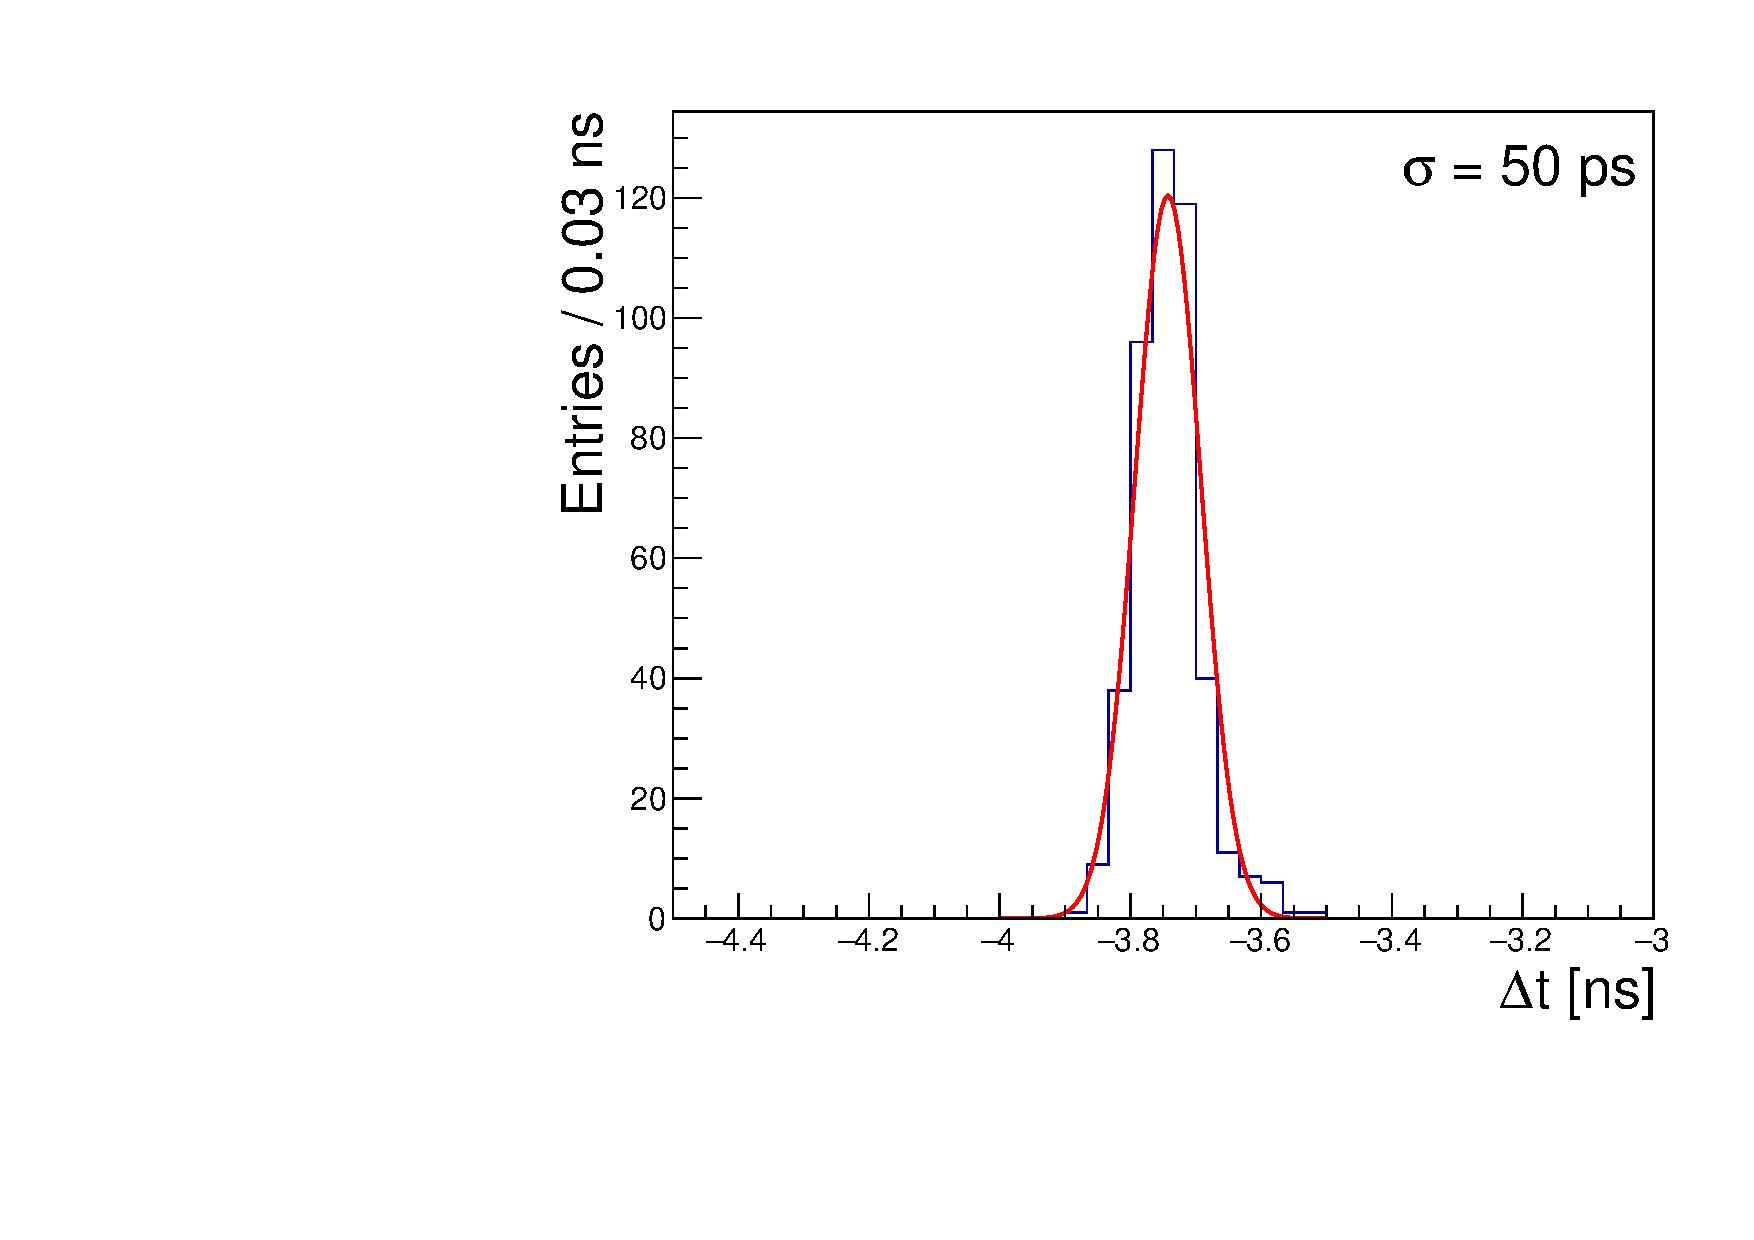
\includegraphics[width=8cm]{Images/exdt/exdtWI.pdf} 
\caption{\small The time distributions obtained using the highest energy pixel (left) and the energy weighted algorithm (right) are shown for one example run. The distributions are
fitted with Gaussian models, and the width parameter of the Gaussian is
displayed on the plot.} 
\label{fig:exdt} 
\end{figure*} 

In Figure~\ref{fig:wtres}, we compare the time resolution for electromagnetic
showers measured using the two methods described above. The time resolution for
the pixel with the largest energy deposit is around $70$~ps and $85$~ps,
depending on the run. Using the energy weighted algorithm improves the time
resolution consistently to about $50$~ps. 

\begin{figure}[htbp] 
\centering
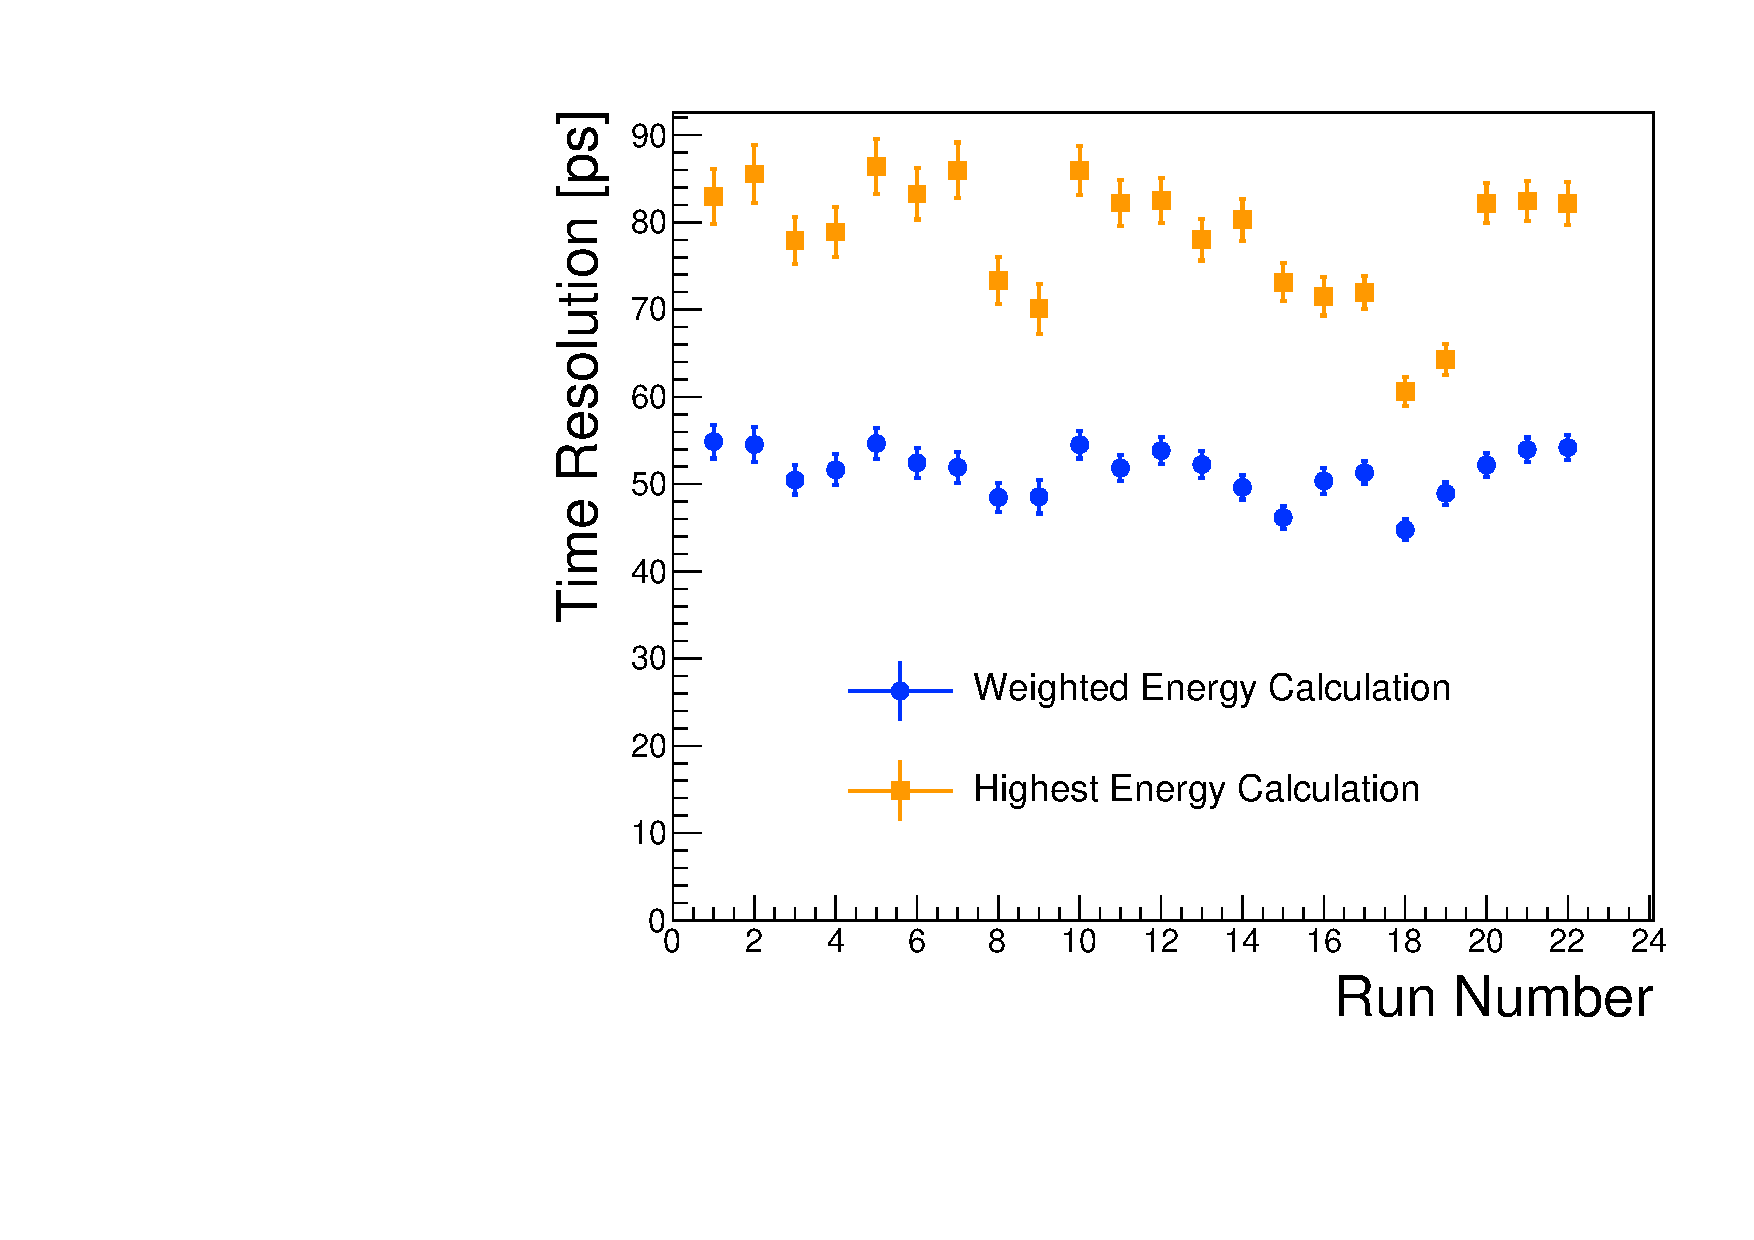
\includegraphics[width=8cm]{Images/wtres/tresperrun.pdf} 
\caption{\small Time resolution found for each run. The time-stamp weighting method consistently results in under $60$~ps. Notice how the highest-signal-pixel method for picking
the time-stamp value is significantly worse.} 
\label{fig:wtres} 
\end{figure} 

We note that the time measurement made using the Photonis MCP-PMT typically exhibit
a dependence on the pulse amplitude or integrated charge. This dependence is
shown on the left of Figure~\ref{fig:dt-int}, and is observed to be
approximately the same for all pixels. We perform a correction to the time
measurement based on the measured integrated charge, and we verify that the
correction does flatten the dependence of the time measurement on the integrated
charge as shown on the right panel of Figure~\ref{fig:dt-int}. After performing
this time measurement correction, the time resolution measurements improve to
about $35$~ps and is shown in Figure~\ref{fig:calib}. We performed two sets of
correction procedures. In one set, labelled as ``Self-Calibrated'', an
independent correction is derived for each run and for each pixel. In the second
set, labelled as ``Calibrated'', a single correction is obtained for each pixel
from a single run, and this correction is applied to all other runs.
Figure~\ref{fig:calib} shows that this single correction is applicable to all
other runs without loss of the precision of the measurements. 

\begin{figure*}[htbp] 
\centering
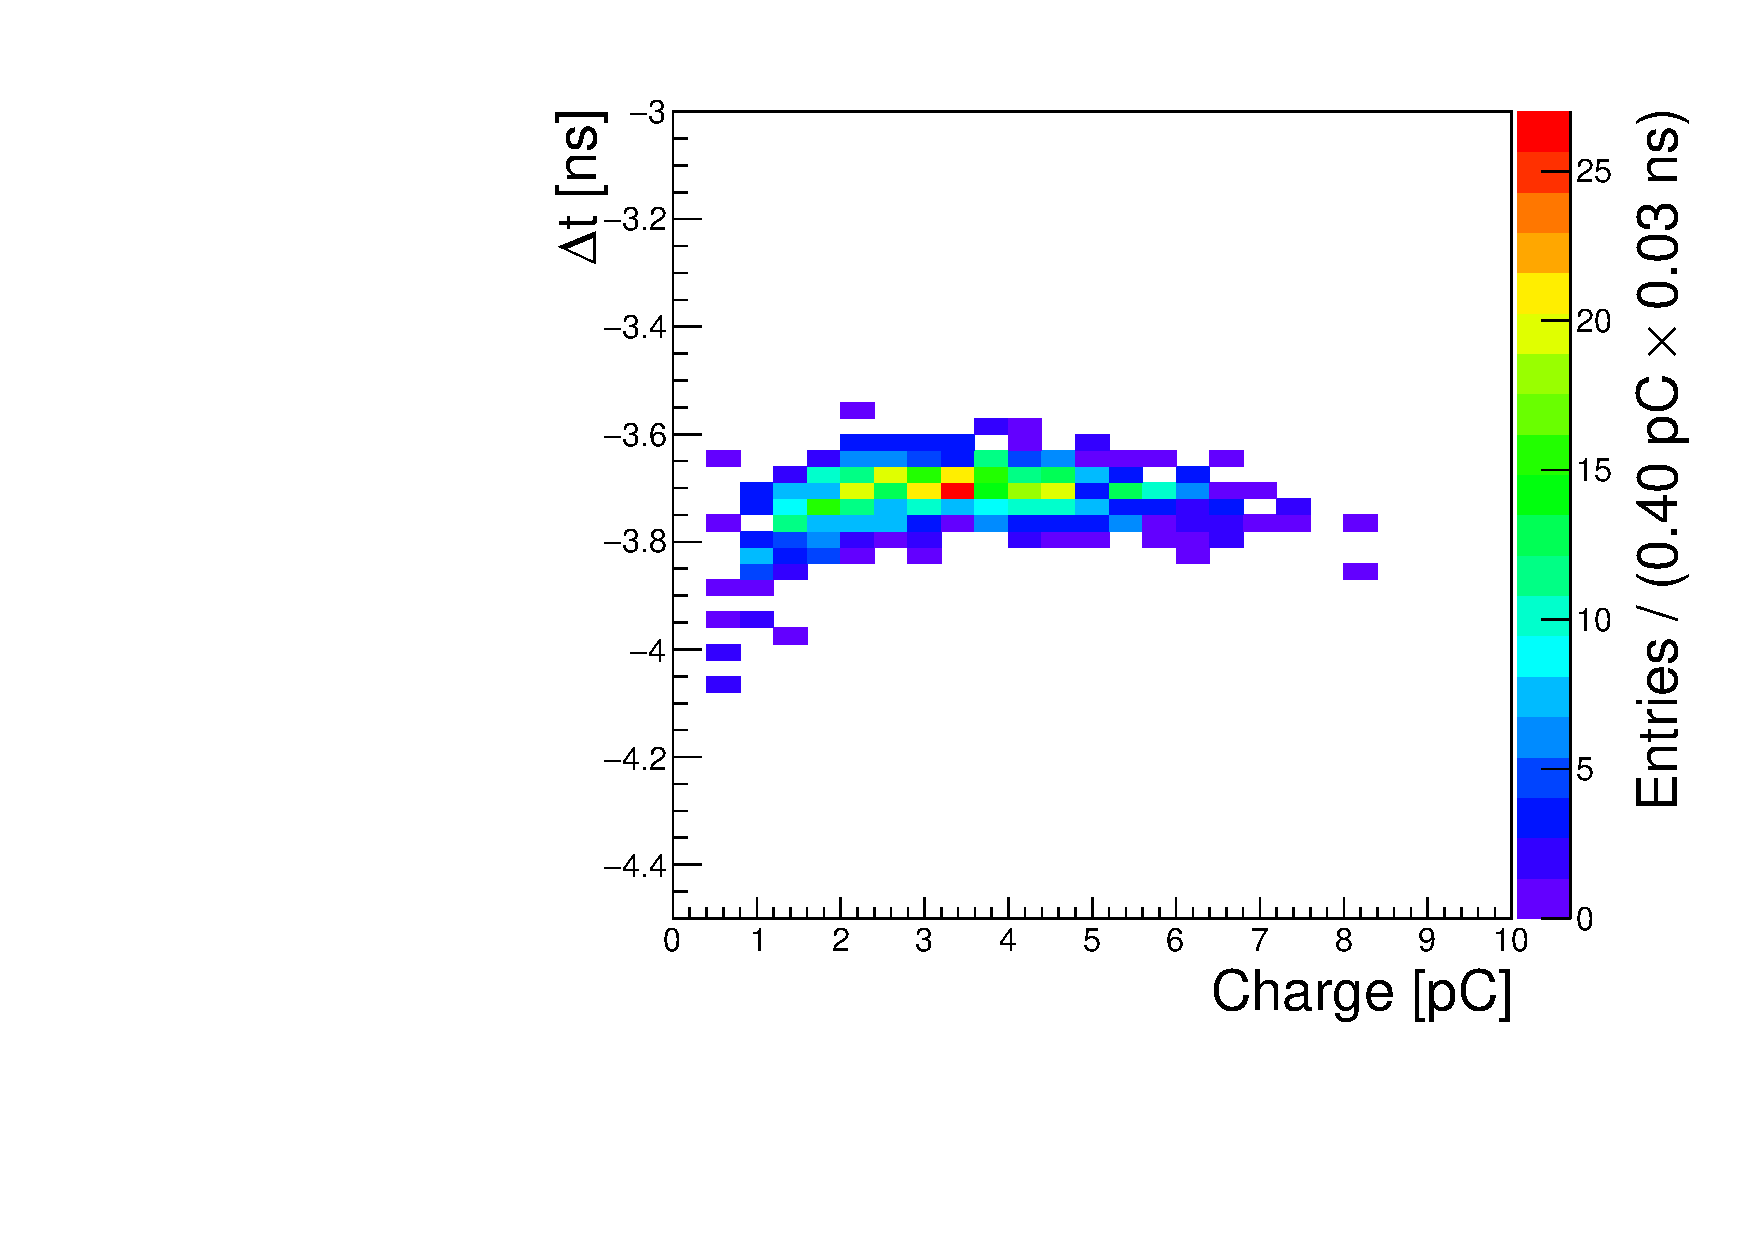
\includegraphics[width=8cm]{Images/dt-int/dtint30_o22.pdf}
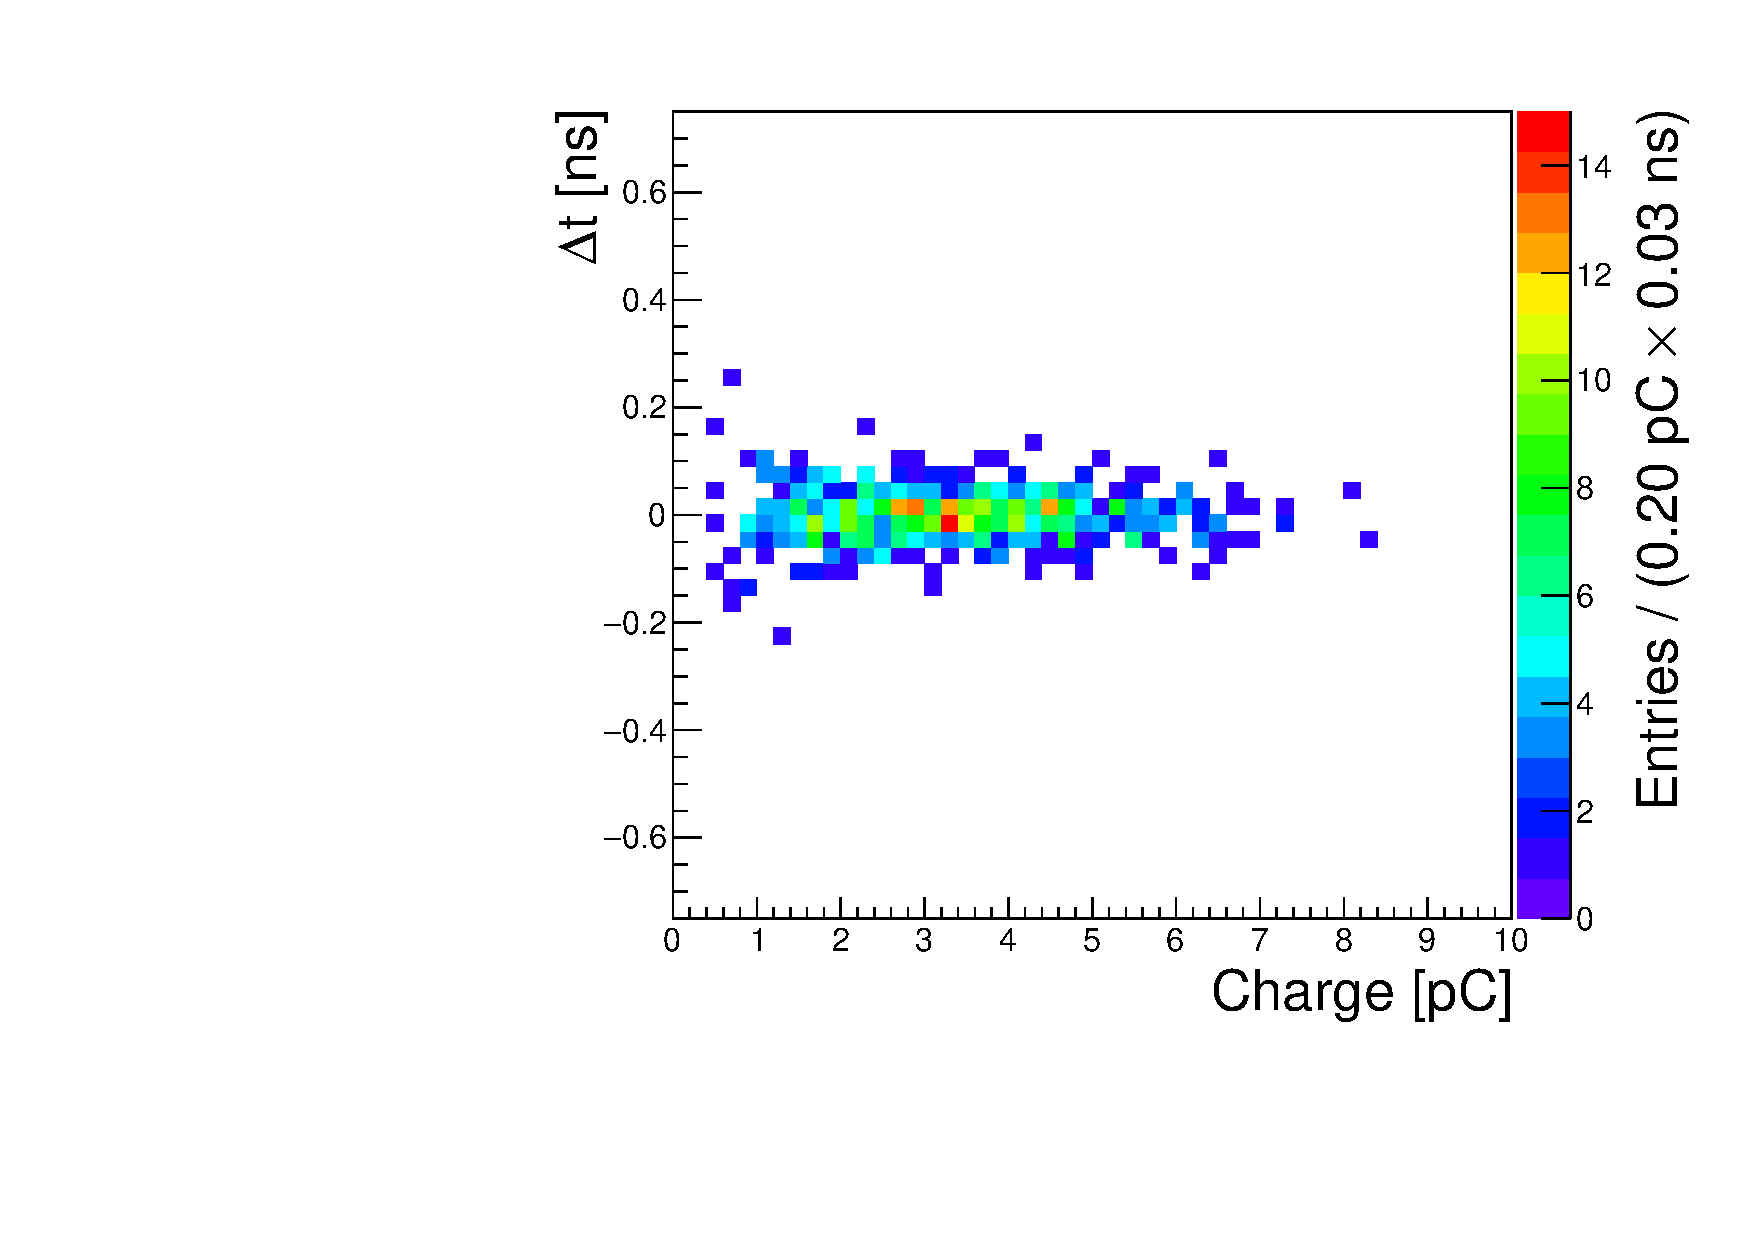
\includegraphics[width=8cm]{Images/dt-int/dtint30_c22.pdf} 
\caption{The correlation between the time measurement and the measured integrated charge is
shown on the left for one example pixel. The same correlation after performing
the time measurement correction is shown on the right. } 
\label{fig:dt-int}
\end{figure*} 

\begin{figure}[htbp] 
\centering
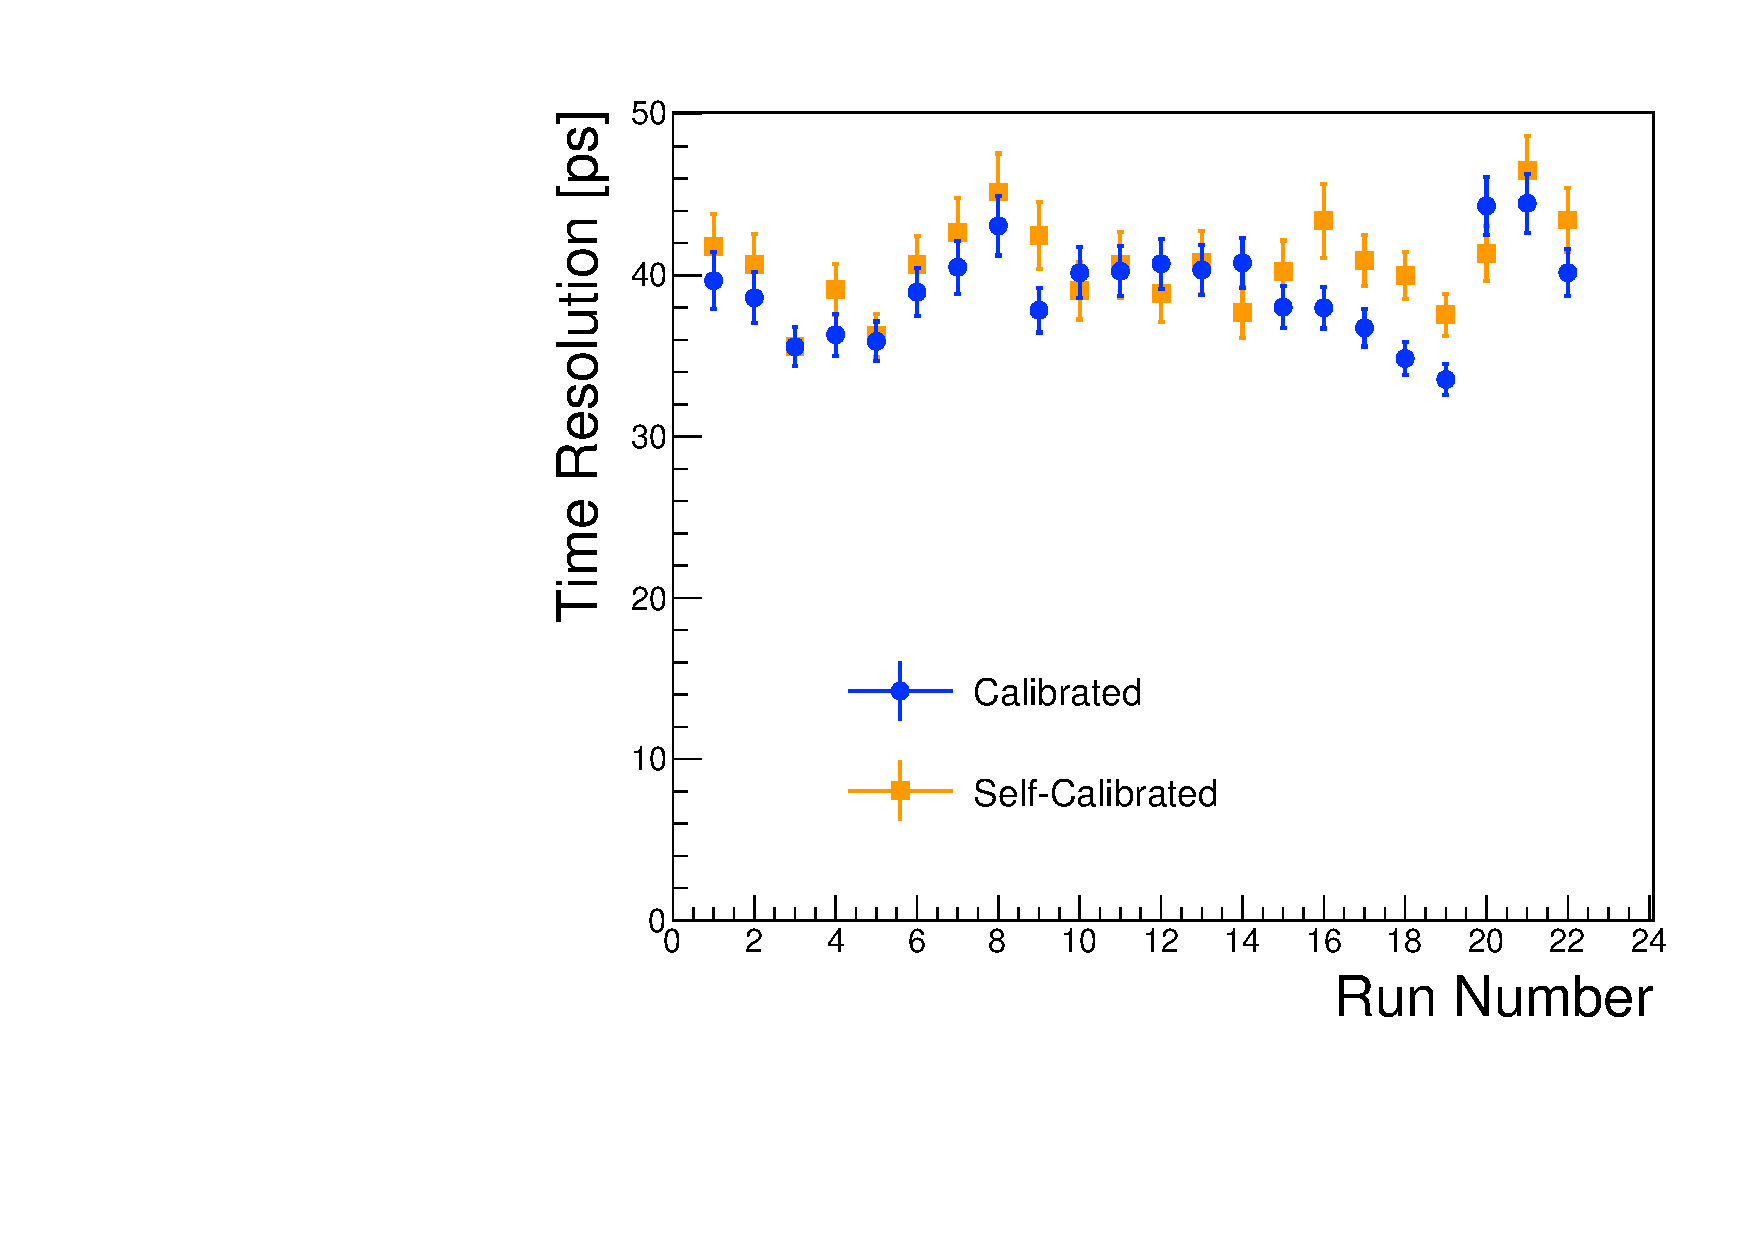
\includegraphics[width=8cm]{Images/calibtres/timerescalib.pdf} 
\caption{ The time resolution of the electromagnetic shower for various runs is
shown after performing the time measurement correction based on the measured
integrated charge. } 
\label{fig:calib} 
\end{figure} 

Finally, we study the dependence of the electromagnetic shower time resolution
as a function of the number of pixels included in the energy-weighted algorithm.
Figure~\ref{fig:sqrtN} shows this dependence for one example run. We observe
that the time resolution improves according to a $1/\sqrt{N}$ scaling up to
about 5--6 pixels, and then becomes flat as we include more pixels. The
initial $1/\sqrt{N}$ scaling is encouraging as it indicates that further
granularity may improve the time resolution. As the majority of the shower is
covered by the pixels closest to the center of the shower, it is not surprising
that we do not observe any improvement from the inclusion of additional pixels.
% because they simply do not contain any additional information about the shower.

\begin{figure}[htbp]
  \centering
  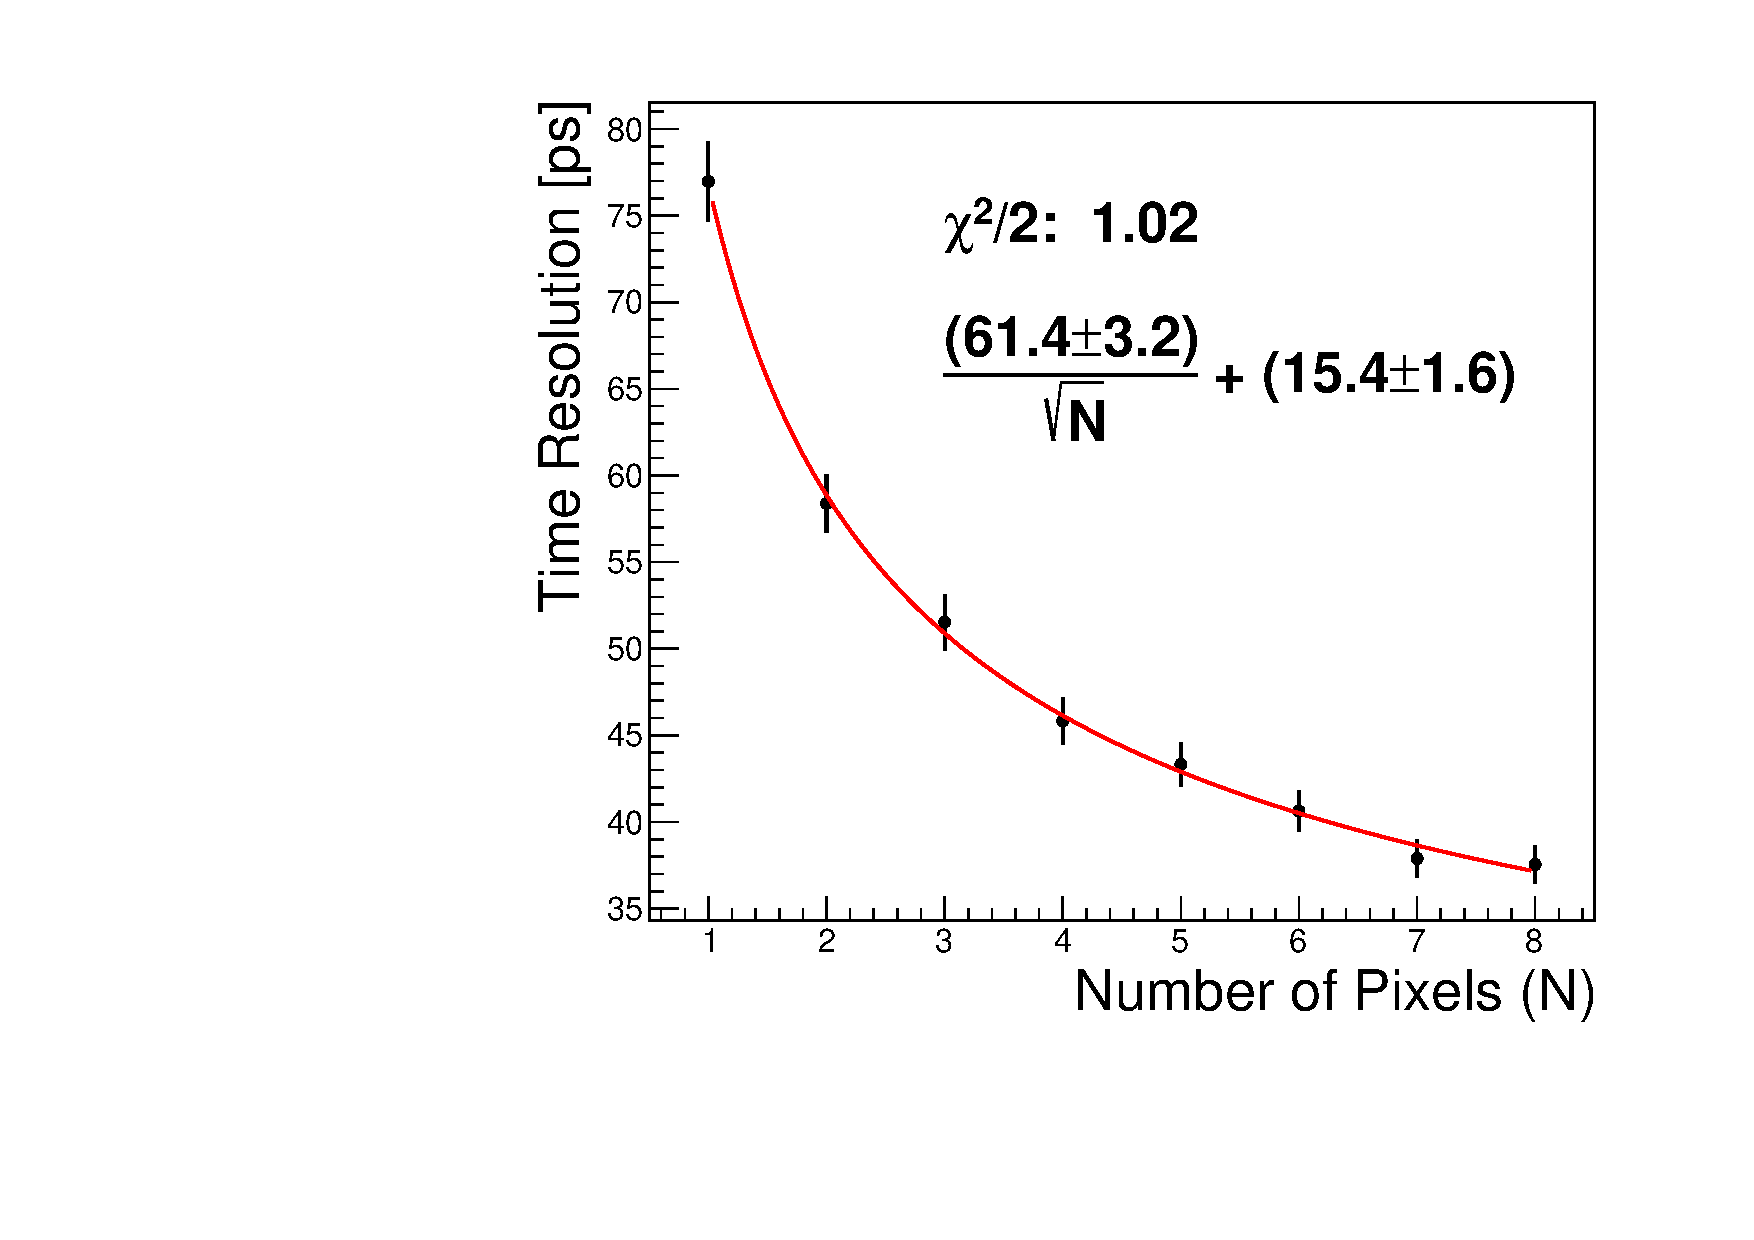
\includegraphics[width=8cm]{Images/sqrtN/t1065_run_38_Dt_IWP.pdf}
  \caption{ The time resolution is plotted as a function of the number of pixels
    included in the energy-weighted algorithm for one example run. }
  \label{fig:sqrtN}
\end{figure}

\section{Summary} 

We report our results on position and time resolution measurements of secondary
emission based calorimeters. As the active material we used Photonis XP85011.
Using a pixelated readout of the MCP-PMT we achieve a highly granular information of
the shower development in the transverse plane. Combining the measurements from
a $3\times3$-channels readout we obtain a sub-millimeter precision for position
measurement, which far exceeds the 6~mm size of individual pixels. We achieve a
time resolution of $30-40$~psec, and show that the time resolution of the
measurements improves with the increase in the number of pixels as $1/\sqrt{N}$.
Our future measurements will include larger prototypes with several layers of
active material, that will allow us to explore the longitudinal development of
the showers.


\section{Acknowledgements} We would like to thank Erik Ramberg for supporting 
our work, and Aria Soha and the FTBF test beam facility for the good beam
delivery and control. Thanks to Ewa Skup and Geoff Savage for help with
operation of Cherenkov counters, and to Todd Nebel for organizing and providing
supporting equipment at FTBF. 

This work is supported by funding from Fermi Research Alliance, LLC under
Contract No. DE-AC02-07CH11359 with the United States Department of Energy, and
from California Institute of Technology High Energy Physics under Contract
DE-SC0011925 with the United States Department of Energy.

\bibliography{PixelMCPPaper2015}{}
\bibliographystyle{ieeetr} \end{document}